\documentclass[
  % 12pt, % set in settings with fontsize package
  % landscape % set with geometry package
  % twoside % set with geometry package
  % draft % "draft" compiles much faster than "final"/!\ do not use final in custom draftmode
  ]{scrartcl}

  % INITIAL IMPORTS: VARIABLES, CONSTANTS, ETC...
\usepackage{luacode} % for 'luacode' environment and '\luastring' macro

% Lua code to record the start time
\begin{luacode*}
    startTime = os.clock()
    endTime = nil
    elapsedTime = nil
\end{luacode*}


%%% Create variables that will be stored in aux file
\providecommand{\myCompileDuration}{0}%
\providecommand{\elapsedInt}{0}%
\providecommand{\elapsedFrac}{0}%

%%% Macro to write to auxiliary file
\makeatletter
\newcommand{\writeToAux}[2]{%
%%% \immediate\write\@auxout: Writes immediately to the .aux file.
%%% \string: Ensures that \ characters are written verbatim to the .aux file.
%%% \gdef: Makes the definition global, so it will work in subsequent runs.
% \immediate%
\protected@write\@auxout{}{\gdef\string#1{#2}}}
\makeatother

%%% Calculate elapsed time at the end of the document
\AtEndDocument{
    \luaexec{
        %-- beware of special characters! need to escape them%
        %-- beware of paragraphs !!!
        %-- Comment can cause issues, always add "--" and keep in separate lines!
        endTime = os.clock()
        %-- Calculate time difference
        elapsedTimeSeconds=endTime-startTime
        elapsedTimeMilliseconds=(elapsedTimeSeconds\%1)*10
        %-- any higher multiplication (100, 1000) and it fails for unknown reason
        %-- integer part
        elapsedInt=math.floor(elapsedTimeSeconds)
        %-- fractional part
        elapsedFrac=math.floor(elapsedTimeMilliseconds)
        %-- Format string
        elapsedIntFormatted=tostring(elapsedInt)
        elapsedFracFormatted=tostring(elapsedFrac)
        %-- Define the elapsed time in a TeX macro
        %-- tex.print("\\gdef\\myCompileDurationTemp{" .. string.format("\%.2f seconds", elapsedTimeSeconds) .. "}")
        %-- Write to the AUX file directly
        f=io.open("auxiliary_files/\jobname.aux","a")
        f:write("\\gdef\\elapsedInt{"..elapsedIntFormatted.."}")
        f:write("\\gdef\\elapsedFrac{"..elapsedFracFormatted.."}")
    }
    %
    \isDraftDebugger{%
        \luaexec{
        % -- Print the values for debugging at document ned
        tex.print("Start Time: " .. string.format("\%.2f", startTime))
        tex.print(" --- ")
        tex.print("End Time: " .. string.format("\%.2f", endTime))
        tex.print(" --- ")
        tex.print("Elapsed Time: " .. string.format("\%.2f", elapsedTimeSeconds))
        }%
    }{}
    % STORE RESULT FOR SUBSEQUENT RUNS
    % \writeToAux{\myCompileDuration}{myCompileDurationTemp}
    % \elapsedInt
    % \elapsedFrac
}

% Overwritten in the article
% Do not use underscores



% Overwritten in the article
% Do not use underscores

\newcommand{\myarticleKeyCore}{} % biblatex key for my article (stripped of prefixes and suffixes, e.g. "article_template"). Leave empty here, else risk of side effects.
\newcommand{\myarticleKey}{%
myarticle:\myarticleKeyCore:\myLanguage%
}% biblatex key for my article

\newcommand{\myMainImg}{} % Main image, if any

\newcommand{\mainSourceKey}{bibliography:source_template} % biblatex key for main source citation

\usepackage{hologo}
\usepackage{ifluatex}
\usepackage{ifxetex}
\usepackage{ifvtex}

%%%%%%%%% VERSIONS
%  THESE VALUES ARE LIKELY TO BE OVERWITTEN DOWNSTREAM

\usepackage{etoolbox} %necessary for booleans
%%% Rules:
% Everything cammelcase!
\newcommand{\createAndSetBoolean}[2]{
  % #1: boolean name
  % #2: set to true or false
  \newbool{#1}\setbool{#1}{#2}
}

\newcommand{\myLanguage}{en}
% Language options: en, fr

% Whether PDF should be in draft or final style
\createAndSetBoolean{isDraft}{false} % true or false
% Whether to go into minimal, high speed mode
\createAndSetBoolean{isMinimal}{true} % true or false
% Whether figures should be included or skipped
\createAndSetBoolean{isIncludeFigures}{true} % true or false
% Whether
\createAndSetBoolean{isPrintVersion}{false} % true or false
\createAndSetBoolean{isDrawRibbons}{false}  % true or false
\createAndSetBoolean{isIncludeMeta}{true} % true or false
\createAndSetBoolean{isIncludeArticleCover}{true} % true or false
\createAndSetBoolean{isIncludeToC}{true}  % true or false
\createAndSetBoolean{isIncludeLoF}{true}  % true or false
\createAndSetBoolean{isIncludeLoT}{true}  % true or false
\createAndSetBoolean{isIncludeLoTB}{true}  % true or false
\createAndSetBoolean{isIncludeBiblio}{true}  % true or false
\createAndSetBoolean{isIncludeGlossary}{true}  % true or false
\createAndSetBoolean{isIncludeAbreviations}{true}  % true or false
\createAndSetBoolean{isPrintUnusedGlossary}{true}  % true or false
\createAndSetBoolean{isPrintUnusedAbreviations}{true}  % true or false
\createAndSetBoolean{isHighlightGlossaryAndAbreviations}{true}  % true or false
\createAndSetBoolean{isIncludeMissingBibEntries}{true}  % true or false
\createAndSetBoolean{hidecontentswitch}{true}  % true or false
\createAndSetBoolean{revealhiddenswitch}{false}  % true or false
% Whether footnotes should be included or ignored
\createAndSetBoolean{isIncludeFootnotes}{true}  % true or false
% Whether citations should be included or ignored
\createAndSetBoolean{isIncludeCitations}{true}  % true or false
% Whether citations should be printed in footnotes
\createAndSetBoolean{isIncludeCitationsInFootnotes}{true}  % true or false
% Whether textboxes should be printed or ignored
\createAndSetBoolean{isIncludeTextBoxes}{true}  % true or false
% Whether textboxes should be printed only at the end of article
\createAndSetBoolean{isMoveTextBoxesToEndOfArticle}{false}  % true or false
% Whether to constrain floats to respective sections
\createAndSetBoolean{isConstrainFloats}{true}  % true or false
% Whether lists items should be inline
\createAndSetBoolean{isCollapseLists}{true}  % true or false
% Whether to include cover image in the article body
\createAndSetBoolean{isIncludeArticleCoverImgInBody}{false}  % true or false
% Whether to include cover image in the article body
\createAndSetBoolean{isCreditsInArticleBody}{true}  % true or false
% Whether to include cover image in the article body
\createAndSetBoolean{isSplitInTwoColumns}{false}  % true or false
% Whether to make whole document in landscape mode or not
\createAndSetBoolean{isLandscapeMode}{false}  % true or false
% Whether to include appendix
\createAndSetBoolean{isIncludeAppendix}{false}  % true or false
% Whether to print custom logs
\createAndSetBoolean{isPrintLogs}{true}  % true or false


%%%% PORTOFOLIO SPECIFIC:
% Whether to add a higher level of organisation as parts to group articles
\createAndSetBoolean{isDivideArticlesIntoParts}{true}  % true or false
% Whether each article should have its own sub TOC/LOT/LOT
\createAndSetBoolean{isIncludePerArticleToC}{true}  % true or false
\createAndSetBoolean{isIncludePerArticleLoF}{true}  % true or false
\createAndSetBoolean{isIncludePerArticleLoT}{true}  % true or false
% Whether each article shows its substance in portfolio
\createAndSetBoolean{isIncludePerArticleSubstance}{true}  % true or false
% Whether the bibliography is split between chapters or grouped at end
\createAndSetBoolean{isSplitBibliographyByChapter}{false}  % true or false






\usepackage{xstring} % Needed for string manipulation

\newcommand{\addonlyfiles}[1]{%
  \def\onlyfiles{#1}%
}


% Create new command: \addContent
\NewDocumentCommand\addContent{
  +m % Arg 1 (Mandatory): Section
  +O{} % Arg 2 (Optional): Language
  }{

    \ifthenelse{\equal{#2}{}}%
      { % IF
        \def\fileAddress{elements/#1/#1.tex}%
      }%
      { % ELSE
        \def\fileAddress{elements/#1/#1\_#2.tex}%
      }%
    % \textcolor{green}{\fileAddress}


    % Update ribbons
    \updateRibbons{Article: \textbf{\myCiteEntry{\myarticleKey}{title}}\ribbonSpacer Section : \textbf{#1}}{#2}

    \IfSubStr{\onlyfiles}{#1}{ %%% only if it is part of \addonlyfiles list
      \InputIfFileExists{\fileAddress}
        {%
           % then
          % Add code here (it is run before file)
        }%
        {%
    %     % else
        \textcolor{myColorDanger}{\Huge #1 #2: CONTENT DOES NOT EXIST}
    %     % ...
        }%
    }

}



%%%%%%%%%%%%%%%%%%%%%%%%%%%%%%%%%%%%%%%%%%%%%%%%%%%%%%%%%%%%%%%%%%%%%%%%%%%%%%

%%%%%% SWITCH MODULE
% https://tex.stackexchange.com/questions/87656/turning-parts-of-text-on-and-off

% new environment for switchable areas
\NewDocumentEnvironment{hidecontent}{O{999}}%
% WARNING: if no argument is provided, content must NOT start with an empty paragraph. If argument is provided, it seems ok, but generally it is better to avoid the empty paragraph.
{%
  \ifnum\version<#1%
  \ifbool{hidecontentswitch}{\comment}%
  \ifbool{revealhiddenswitch}{\color{hideEnvColor}%
  }%
  \else%
  \fi%
  }%
{%
  \ifnum\version<#1%
  \ifbool{hidecontentswitch}{\endcomment}%
  \else%
  \fi%
  }%

% without color option (basic)
\NewDocumentEnvironment{hidecontentbasic}{O{999}}%
% WARNING: if no argument is provided, content must NOT start with an empty paragraph. If argument is provided, it seems ok, but generally it is better to avoid the empty paragraph.
{%
  \ifnum\version<#1%
  \ifbool{hidecontentswitch}{\comment}%
  \else%
  \fi%
  }%
{%
  \ifnum\version<#1%
  \ifbool{hidecontentswitch}{\endcomment}%
  \else%
  \fi%
  }%

%that's it ! now I need to use
% \begin{hidecontent}
% \end{hidecontent}


% with color option
\newcommand{\hide}[2][999]{%
    \ifnum\version<#1%
     \ifbool{hidecontentswitch}{}{%
      \ifbool{revealhiddenswitch}{%
      \ignorespaces\textcolor{hideColor}{%
          #2}}{%
          \ignorespaces#2}%
     }%
     \else%
     #2%
    \fi%
}%

% without color option (basic)
\newcommand{\hidebasic}[2][999]{%
    \ifnum\version<#1%
     \ifbool{hidecontentswitch}{}{%
      \ignorespaces#2%
     }%
    \else%
     #2%
    \fi%
}%

%%%% Shorthand to check if portfolio (yes) or article (no) document
\newcommand{\isPortfolio}[2]{%
  \ifthenelse{\equal{\jobname}{\detokenize{portfolio_document}}}
  {#1}
  {#2}
}%

%%%% Shorthand to check if article (yes) or portfolio (no) document
\newcommand{\isArticle}[2]{%
  \ifthenelse{\equal{\jobname}{\detokenize{document}}}
  {#1}
  {#2}
}%

%%%% Shorthand to check if print version
\newcommand{\isPrint}[2]{%
  \ifthenelse{\boolean{isPrintVersion}}%
  {#1}%
  {#2}%
}

%%%%%%%%%%%%%%%%%%%%%%%%%%%%%%%%%%%%%%%%%%%%%%%%
% MAIN VARIABLES %%%%%%%%%%%%%%%%%%%%%%%%%%%%%%%
%%% DEFINE MAIN VARIABLES HERE
%
%
%%% The article's identifying key. "\myArticleKey" command will be generated from it.
% Ensure that this key, this filename, and containing foldername match
\renewcommand{\myarticleKeyCore}{%
    \detokenize{article_tutorial}%
}
%%% The chosen language
\renewcommand{\myLanguage}{en}

% Main image to illustrate the article, if any (avoid underscores or other special characters)
\renewcommand{\myMainImg}{./figures/example-image.jpg}

%%% The main source's key
\renewcommand{\mainSourceKey}{%
bibliography:source_template%
}%
 % /!\ UPDATE HERE
%%%%%%%%%%%%%%%%%%%%%%%%%%%%%%%%%%%%%%%%%%%%%%%%


%%% to run individuals fragments
% Include only choosen sections
\newcommand{\filesToAdd}{
  substance,
  body
}



%%% choose which appendix entries to include
\newcommand{\appendixList}
{% leave no spaces to be able to detect when list is empty
    appendix_a,%
    appendix_b%
}

\setbool{isMinimal}{false} % overwrites most booleans below
\setbool{isDraft}{false} % true or false
\setbool{isPrintVersion}{false} % true or false
\setbool{isDrawRibbons}{false} % true or false
\setbool{isIncludeMeta}{true} % true or false
\setbool{isIncludeArticleCover}{true} % true or false
\setbool{isIncludeToC}{true} % true or false
\setbool{isIncludeLoF}{true} % true or false
\setbool{isIncludeLoT}{true} % true or false
\setbool{isIncludeLoTB}{true} % true or false
\setbool{isIncludeBiblio}{true} % true or false
\setbool{isIncludeGlossary}{true} % true or false
\setbool{isIncludeAbreviations}{true} % true or false
\setbool{isPrintUnusedGlossary}{true} % true or false
\setbool{isPrintUnusedAbreviations}{true} % true or false
\setbool{isHighlightGlossaryAndAbreviations}{true}  % true or false
\setbool{isIncludeMissingBibEntries}{false} % true or false
\setbool{isIncludeFootnotes}{true} % true or false
\setbool{isIncludeCitations}{true} % true or false
\setbool{isIncludeCitationsInFootnotes}{true} % true or false
\setbool{isIncludeTextBoxes}{true} % true or false
\setbool{isMoveTextBoxesToEndOfArticle}{false}  % true or false
\setbool{isConstrainFloats}{false}  % true or false
\setbool{isIncludeArticleCoverImgInBody}{true}  % true or false
\setbool{isCreditsInArticleBody}{true}  % true or false
\setbool{isSplitInTwoColumns}{false} % true or false
\setbool{isLandscapeMode}{false} % true or false
\setbool{isIncludeAppendix}{true} % true or false
\setbool{isPrintLogs}{true} % true or false



%%% To toggle out part(s) of the article with a switch:
% change true/false here to control behavior
\setbool{hidecontentswitch}{false} %true (exclude) or false (include)
\setbool{revealhiddenswitch}{true} %true (color) or false (no color) - (hidecontentswitch must be ¨false¨)
% pick version to print, more is included as the number goes up:
\newcommand\version{0}
% levels:
% empty = 999 <- exclude all
% version 0 <- exlude all excpect hide's with a param 0
% version 1 <- exlude all except hide's with param 0 or 1
% version 2 <- exlude all except hide with param 1, 2
% version n <- exlude all except hide with param 1, 2, ..., n

%SETTINGS

% \usepackage{ifthen}
\usepackage{xifthen}
\usepackage{lipsum} % Lorem Ipsum



\newcommand{\setMinimalMode}
{
    \isMinimal
    {

        \ifthenelse{\equal{\jobname}{\detokenize{portfolio_document}}}
        {
            \includeonly{ %to run individuals fragments
            % elements/portfolio_meta_data/portfolio_meta_data,
            % elements/portfolio_title_page/portfolio_title_page,
            % elements/preface/preface
            }
        }
        {
            \addonlyfiles{
                % substance,
                % glossary,
                % abreviations,
                body
            }
        }

        % \setbool{isDraft}{true} % true or false
        \setbool{isPrintVersion}{false} % true or false
        \setbool{isDrawRibbons}{false} % true or false
        \setbool{isIncludeMeta}{false} % true or false
        \setbool{isIncludeArticleCover}{false} % true or false
        \setbool{isIncludeToC}{false} % true or false
        \setbool{isIncludeLoF}{false} % true or false
        \setbool{isIncludeLoT}{false} % true or false
        \setbool{isIncludeLoTB}{false} % true or false
        \setbool{isIncludeBiblio}{false} % true or false
        \setbool{isIncludeGlossary}{false} % true or false
        \setbool{isIncludeAbreviations}{false} % true or false
        \setbool{isPrintUnusedGlossary}{false} % true or false
        \setbool{isPrintUnusedAbreviations}{false} % true or false
        \setbool{isHighlightGlossaryAndAbreviations}{false}  % true or false
        \setbool{isIncludeMissingBibEntries}{false} % true or false
        \setbool{isIncludeFootnotes}{false} % true or false
        \setbool{isIncludeCitations}{false} % true or false
        \setbool{isIncludeCitationsInFootnotes}{false} % true or false
        \setbool{isIncludeTextBoxes}{false} % true or false
        \setbool{isMoveTextBoxesToEndOfArticle}{false}  % true or false
        \setbool{isConstrainFloats}{false}  % true or false
        \setbool{isIncludeArticleCoverImgInBody}{false}  % true or false
        \setbool{isCreditsInArticleBody}{false}  % true or false
        \setbool{isSplitInTwoColumns}{false} % true or false
        \setbool{isLandscapeMode}{false} % true or false
        \setbool{isIncludeAppendix}{false} % true or false

        %%%% PORTOFOLIO SPECIFIC:
        \setbool{isIncludePerArticleToC}{false} % true or false
        \setbool{isIncludePerArticleLoF}{false} % true or false
        \setbool{isIncludePerArticleLoT}{false} % true or false
        \setbool{isIncludePerArticleSubstance}{false} % true or false
        \setbool{isSplitBibliographyByChapter}{false}  % true or false

        %%%% OTHER SETTINGS:
        \pagecolor{black}% bg color
        \color{white}% text color
    }
    {}
}

\AfterPreamble{
    \setMinimalMode
}

%%% ===== MACRO TO RUN CONTENTS ONLY IN DRAFT VERSION
\newcommand{\isMinimal}[2]{%
    \ifthenelse{\boolean{isMinimal}}%
    {#1}%
    {#2}%
}

% make sure to update language in document as well
% ENGLISH (EN)
\ifthenelse{\equal{\myLanguage}{en}}{
  \usepackage[english]{babel}
  \usepackage[en-GB]{datetime2}
  \newcommand{\myLanguageLong}{english}
  %
  %
  %
  \newcommand{\TEXTcover}{Cover}
  \newcommand{\TEXTtoc}{Table of Contents}
  \newcommand{\TEXTlof}{List of Figures}
  \newcommand{\TEXTlot}{List of Tables}
  \newcommand{\TEXTpToc}{Partial Table of Contents}
  \newcommand{\TEXTpLof}{Partial List of Figures}
  \newcommand{\TEXTpLot}{Partial List of Tables}
  \newcommand{\TEXTlotb}{List of Textboxes}
  \newcommand{\TEXTmainSource}{Main source}
  \newcommand{\TEXTtextbox}{Textbox}
  \newcommand{\TEXTbibliography}{Bibliography}
  \newcommand{\TEXTchapter}{Article}
  \newcommand{\TEXTacknowledgements}{Acknowledgements}
  \newcommand{\TEXTpreface}{Preface}
  \newcommand{\TEXTpostface}{Postface}
  \newcommand{\TEXTquotation}{Quotation}
  \newcommand{\TEXTby}{by}
}{}%

% FRENCH (FR)
\ifthenelse{\equal{\myLanguage}{fr}}{
  \usepackage[french]{babel}
  \usepackage[french]{datetime2}
  \newcommand{\myLanguageLong}{french}
  %
  %
  %
  \newcommand{\TEXTcover}{Couverture}
  \newcommand{\TEXTtoc}{Table des Matières}
  \newcommand{\TEXTlof}{Liste des Figures}
  \newcommand{\TEXTlot}{Liste des Tableaux}
  \newcommand{\TEXTpToc}{Table Partielle des Matières}
  \newcommand{\TEXTpLof}{Liste Partielle des Figures}
  \newcommand{\TEXTpLot}{Liste Partielle des Tableaux}
  \newcommand{\TEXTlotb}{Liste des Notes}
  \newcommand{\TEXTmainSource}{Source principale}
  \newcommand{\TEXTtextbox}{Encadré}
  \newcommand{\TEXTbibliography}{Bibliographie}
  \newcommand{\TEXTchapter}{Article}
  \newcommand{\TEXTacknowledgements}{Remerciements}
  \newcommand{\TEXTpreface}{Avant-propos}
  \newcommand{\TEXTpostface}{Postface}
  \newcommand{\TEXTquotation}{Quotation}
  \newcommand{\TEXTby}{par}
}{}%

% \DTMlangsetup{ord=raise,showdayofmonth=false}

\usepackage[inline]{enumitem} % to customize lists

% Command to create a hidden item that takes no space in a list
\def\hiddenitem{%
    \item[]%
    \vskip-\baselineskip%
    \vskip-\parsep%
    \vskip-\itemsep%
}

% EXPANDED LIST WITH LINE BREAKS BETWEEN ITEMS
\newlist{myListMeta}{enumerate}{1}
\setlist[myListMeta]{
    label={},
    align=right, % label alignment
    % labelwidth=0.25cm,
    topsep=0pt, % reduce space above list
    itemsep=0pt, % Sets the space between items
    parsep=0pt, % Sets the space between paragraphs within the items
    leftmargin=100pt, % * or 0pt
    labelsep=10pt, % Space between the bullet and the item text
}

% COLLAPSED LIST WITH INLINE ITEMS
\newlist{myListMetaCollapsed}{enumerate*}{1}
\setlist[myListMetaCollapsed]{
% label=(\textbf{\arabic*})
}



\newenvironment{customlist} % Define the new environment
  {
    \ifthenelse{\boolean{isCollapseLists}}% Check if the argument is "enumerate"
    {\begin{myListMetaCollapsed}}% If yes, start
    {\begin{myListMeta}}%
    }%
  {%
  \ifthenelse{\boolean{isCollapseLists}}% Check if the argument is "enumerate"
  {\end{myListMetaCollapsed}}% If yes, end
  {\end{myListMeta}}%
  }%


% LIST STYLES USED INSIDE ARTICLE
% \newlist{<list name>}{<bases>}{<max depth>}
\newlist{myListEnumerate}{enumerate}{1}
\newlist{myListItemize}{itemize}{1}
% Define a shared macro for list settings
\def\myListAlign{right}
\def\myListTopsep{0pt} % space above list
\def\myListItemsep{8pt} % space between items
\def\myListParsep{0pt} % space between paragraphs within the items
\def\myListLeftmargin{10pt} % space on the left. * or 0pt
\def\myListLabelsep{10pt} % space between the bullet and the item text
%
\setlist[myListEnumerate]{
    label=({\arabic*}),
    align=\myListAlign, % label alignment
    % labelwidth=0.25cm,
    topsep=\myListTopsep, % space above list
    itemsep=\myListItemsep, % space between items
    parsep=\myListParsep, % space between paragraphs within the items
    leftmargin=\myListLeftmargin, % space on the left. * or 0pt
    labelsep=\myListLabelsep, % space between the bullet and the item text
}
\setlist[myListItemize]{
    label={--},
    align=\myListAlign, % label alignment
    % labelwidth=0.25cm,
    topsep=\myListTopsep, % space above list
    itemsep=\myListItemsep, % space between items
    parsep=\myListParsep, % space between paragraphs within the items
    leftmargin=\myListLeftmargin, % space on the left. * or 0pt
    labelsep=\myListLabelsep, % space between the bullet and the item text
}

\usepackage[dvipsnames]{xcolor} % to color comments
% Command to set background color
\usepackage[breakable, skins]{tcolorbox}

\usepackage{transparent}


\definecolor{myColorPrimary}{rgb}{0.3,0.2,0.2}
\definecolor{myColorSecondary}{rgb}{0.1,0.3,0.5}
\definecolor{myColorSuccess}{rgb}{0,1,0}
\definecolor{myColorWarning}{rgb}{1,0.5,0}
\definecolor{myColorDanger}{rgb}{1,0,0}
\definecolor{myGrayDark}{gray}{0.25}
\definecolor{myGrayMed}{gray}{0.5}
\definecolor{myGrayLight}{gray}{0.9}
\definecolor{bgColor}{rgb}{1,1,1}
\definecolor{textColor}{rgb}{0,0,0}
\definecolor{draftBgColor}{rgb}{0.1,0.05,0}
\definecolor{draftTextColor}{RGB}{255,255,255}


% Hidden content colors
\definecolor{hideColor}{rgb}{1,0.5,0.5}
\definecolor{hideEnvColor}{rgb}{0.5,1,0.5}


\colorlet{sectionHeaderColor}{myGrayDark}

\definecolor{sectionDraftContentsBgColor}{rgb}{0.9, 0.7, 0.5}
\colorlet{sectionFinalContentsBgColor}{bgColor}

\pagecolor{bgColor} % Set your desired background color here
\color{textColor} % Set your desired default text color here



%%%%%% Font parameters

\usepackage[T1]{fontenc} % for proper enconding of accents that can be copy pasted
\usepackage[utf8]{inputenc}
\usepackage{fontspec} % Allows for custom fonts (compatible with XeLaTeX or LuaLaTeX; but not with pdfLaTeX)
\usepackage[fontsize=12pt]{fontsize} % Set font size
\usepackage{unicode-math} %
% Set main font with fontspec (if all off, default to Computer Modern)
% \setmainfont{Cambria}
% \setmainfont{Arial}
% \setmainfont{Times New Roman}
% \setmainfont{Helvetica}
% \usepackage{helvet} % use helvetica alternative

% WHEN SETTING FONT FROM A FILE, YOU CAN SPECIFY IT LIKE THIS IF IT IS FAILING
% \setmainfont[
%     Path = /your/font/path/,
%   Extension = .otf ,
%   BoldFont = HelveticaNeueLTPro-Md.otf ,
% ]{HelveticaNeueLTPro-Roman.otf}


% \usepackage{ebgaramond} % Use the EB Garamond font (pdfLaTeX compatible)

%%% use sans serif text
% \renewcommand{\familydefault}{\sfdefault}

%%% use use dyslexic friendly font:
% \setmainfont{Open Dyslexic} % must first install on computer to work

%%% STANDARD WAY TO SET FONTS
% \setromanfont{Times New Roman}
% \setsansfont{Arial}
% \setmonofont{Consolas}[Scale=0.9]
% \setmathfont{Latin Modern Roman}


%%% MY WAY TO SET FONTS
\newcommand{\applyFonts}[2]{%
    % #1 first option
    % #2 backup
    \IfFontExistsTF{#1}
    {%
        \setmainfont{#1}%
    }%
    {% Fallback option
        \setmainfont{#2}%
    }%
}

%%%%%% SETTING FONTS WITH BACKUPS IF NOT AVAILABLE
%%% MAIN FONT
\newcommand{\myMainFont}{Helvetica}
\newcommand{\myMainFontBackup}{Arial}
\newcommand{\setMainFont}{%
    %%% Run immediately after \begin{document}, similar to \AtBeginDocument but the latter is outdated
    \isMinimal% check if in minimal mode
    {}% if yes, do not change font from default to speed up compilation
    {%
        \AfterEndPreamble{
            \applyFonts{\myMainFont}{\myMainFontBackup}
        }%
    }%
}%

%%% SET DEFAULT FONT
\setMainFont%



%%% DRAFT MAIN FONT
\newcommand{\myDraftFont}{Open Dyslexic}
\newcommand{\myDraftFontBackup}{Times New Roman}
\newcommand{\setDraftFont}{%
    %%% Run immediately after \begin{document}, similar to \AtBeginDocument but the latter is outdated
    \isMinimal% check if in minimal mode
    {}% if yes, do not change font from default to speed up compilation
    {%
        \AfterEndPreamble{
            \applyFonts{\myDraftFont}{\myDraftFontBackup}
        }%
    }%
}%


%%% TITLE FONT
\newcommand{\myTitleFont}{Times New Roman}
\newcommand{\myTitleFontBackup}{Times New Roman}
\newcommand{\setTitleFont}{%
    \isMinimal% check if in minimal mode
    {}% if yes, do not change font from default to speed up compilation
    {%
        \applyFonts{\myTitleFont}{\myTitleFontBackup}%
    }%
}%

%%% SUBTITLE FONT
\newcommand{\mySubtitleFont}{Times New Roman}
\newcommand{\mySubtitleFontBackup}{Times New Roman}
\newcommand{\setSubtitleFont}{%
    \isMinimal% check if in minimal mode
    {}% if yes, do not change font from default to speed up compilation
    {%
        \applyFonts{\mySubtitleFont}{\mySubtitleFontBackup}%
    }%
}%


%%%% Page measurements and spacing

\usepackage{geometry}

\ifthenelse{\boolean{isLandscapeMode}}
{%
  \geometry{landscape=true}%
}
{%
  \geometry{landscape=false}%
}

\newcommand{\myWidthDigital}{150mm}
\newcommand{\myTopDigital}{25mm}
\newcommand{\myBottomDigital}{25mm}
\newcommand{\myLeftDigital}{25mm}
\newcommand{\myRightDigital}{25mm}
\newcommand{\myBindingOffsetDigital}{0mm}

\newcommand{\myWidthPrint}{150mm}
\newcommand{\myTopPrint}{25mm}
\newcommand{\myBottomPrint}{25mm}
\newcommand{\myLeftPrint}{25mm}
\newcommand{\myRightPrint}{25mm}
\newcommand{\myBindingOffsetPrint}{8mm}
% DIMENSIONS FOR DIGITAL VERSION
\geometry{
  a4paper,
  width=\myWidthDigital,
  top=\myTopDigital,
  bottom=\myBottomDigital,
  left=\myLeftDigital,
  right=\myRightDigital,
  bindingoffset=\myBindingOffsetDigital,
  twoside % must be true for other features
}
\savegeometry{digital}


% DIMENSIONS FOR PRINTED VERSION
\newgeometry{
  a4paper,
  width=\myWidthPrint,
  top=\myTopPrint,
  bottom=\myBottomPrint,
  left=\myLeftPrint,
  right=\myRightPrint,
  bindingoffset=\myBindingOffsetPrint,
  twoside % must be true for other features
}
\savegeometry{print}


\newcommand{\myGeometrySettingsInfo}{%
text width:\isPrint{\myWidthPrint}{\myWidthDigital};
top margin:\isPrint{\myTopPrint}{\myTopDigital};
bottom margin:\isPrint{\myBottomPrint}{\myBottomDigital};
left margin:
\isPrint{\myLeftPrint}{\myLeftDigital};
right margin:
\isPrint{\myRightPrint}{\myRightDigital};
binding offset:
\isPrint{\myBindingOffsetPrint}{\myBindingOffsetDigital}
}

\usepackage{setspace} % to change spacing between lines
% \onehalfspacing % or
%\singlespacing % or
\doublespacing %
\parskip=1em % spacing between paragraphs (0pt plus 1pt default)
\parindent=15pt % indent at start of each paragraph (15 default)
%%%%



\usepackage{scrextend} %%% Add margins to blocks of text

% \pagestyle{empty}
% \pagestyle{headings}

\usepackage{fancyhdr}
% \pagestyle{fancy} % Enable the fancy page style




\fancypagestyle{styleDigital}{
  \fancyhf{}% Clear header/footer
  % O = odd; E = even; L/R/C = left/right/center
  \fancyhead[RO, RE]{\myArticleTitle}
  \fancyhead[LO, LE]{\myPrintOrDigitalMarker}
  \fancyhead[CO, CE]{
    % \verticalCenterIcon{\includegraphics[scale=0.05]{../../articles_common_files/assets/icons/placeholder.png}}
  }
  % \fancyhead[CO, CE]{\textcolor{myColorPrimary}{\hyperlink{toc}{\leftmark}}}
  \fancyfoot[RO, RE]{
    \textcolor{myColorPrimary}{
      % \hyperlink{title}{\myCiteEntry{\myarticleKey}{author}}
    }
    \myAbsolutePagination
  }
  \fancyfoot[CE, CO]{
    \myRelativePagination
  }
}

%%% DEFINE ANOTHER STYLE BASED ON THIS ONE
\fancypagestyle{styleDigital-NoPage}[styleDigital]{
\fancyfoot[]{} % empty footer
\fancyfoot[RO, RE]{\myAbsolutePagination}
\fancyfoot[LO, LE]{\isDraft{\color{myColorWarning}page without pagination in final v.}{}}
}



\fancypagestyle{stylePrint}{
  \fancyhf{}% Clear header/footer
  % O = odd; E = even; L/R/C = left/right/center
  % HEAD
  \fancyhead[RO, LE]{\myArticleTitle}
  % \fancyhead[LO, RE]{\textcolor{myColorPrimary}{\hyperlink{toc}{\leftmark}}}

  % FOOT
  \fancyfoot[LO, RE]{
    % \textcolor{myColorPrimary}{\hyperlink{title}{\myCiteEntry{\myarticleKey}{author}}}
    \myAbsolutePagination
     }
  \fancyfoot[RO, LE]{
    \textcolor{myColorPrimary}{\myRelativePagination}
    }
  \fancyfoot[CO]{
    % \verticalCenterIcon{\includegraphics[scale=0.05]{../../articles_common_files/assets/icons/placeholder.png}}
    \isDraft{\textcolor{myColorWarning}{ODD (RIGHT)}{}}
  }
  \fancyfoot[CE]{
    % \verticalCenterIcon{\includegraphics[scale=0.05]{../../articles_common_files/assets/icons/placeholder.png}}
    \isDraft{\textcolor{myColorWarning}{EVEN (LEFT)}{}}
  }
}

%%% DEFINE ANOTHER STYLE BASED ON THIS ONE
\fancypagestyle{stylePrint-NoPage}[stylePrint]{
  \fancyfoot[LO,RE, RO, LE]{} % empty footer
  \fancyfoot[LO, RE]{\myAbsolutePagination}
  \fancyfoot[RO, LE]{\isDraft{\color{myColorWarning}page without pagination in final v.}{}}
}


\newcommand{\verticalCenterIcon}[1]{
    \raisebox{-0.5\height}{%center vertically in line
    \scalebox{-1}[1]{%horizontal flipping
      #1
    }
  }
}

%%% Relative pagination (within article)
\newcommand{\myRelativePagination}{%
  \isDraft
  {\hyperlink{toc}{\textcolor{myGrayMed}{\thepage}} \textcolor{myColorPrimary}{out of\totalPagesInArticleBody}}%
  {
    \textcolor{myColorPrimary}{\hyperlink{toc}{\thepage}}%
  }
}

%%% Absolute pagination (whole document)
\newcommand{\myAbsolutePagination}{%
  \isDraft{\textcolor{myColorPrimary}{Absolute page: \textcolor{myGrayMed}{\abspagenumber}/\ztotpages}}{}%
}

%%% Article title
\newcommand{\myArticleTitle}{%
  \hyperlink{\myarticleKey}{\textcolor{myColorPrimary}{\setTitleFont\citefield{\myarticleKey}{title}}}%
}

%%% Print/Digital marker
\newcommand{\myPrintOrDigitalMarker}{%
  \isDraft{%
  \color{myColorWarning}\isPrint{PRINT VERSION}{DIGITAL VERSION}
  }{}
}



% to exclude "chapter #" from footer:
% \renewcommand{\chaptermark}[1]{\markboth{\MakeUppercase{#1}}{}} %remove \makeuppercase{} to keep it normal case

% change ruler style and color
\renewcommand{\headrule}{\hbox to\headwidth{\color{myColorPrimary}\leaders\hrule height \headrulewidth\hfill}}
\renewcommand{\footrule}{\hbox to\headwidth{\color{myColorPrimary}\leaders\hrule height \headrulewidth\hfill}}

% set ruler dimensions
\renewcommand{\headrulewidth}{0pt}
\renewcommand{\footrulewidth}{0pt}
\setlength{\headheight}{15pt}


\fancyheadoffset{0cm}


\usepackage{sectsty}
\sectionfont{\centering} % center section titles

% Used in all indivual article sections except the article title
\newcommand{\mySectionTitleLinker}{}
\newcommand*{\mySectionTitle}[1]{
    \renewcommand{\mySectionTitleLinker}{%
        \myarticleKeyCore:\detokenize{#1}%
    }
    \phantomsection % ensures linking with hyperref to exact page
    \hypertarget{\mySectionTitleLinker}{}
    % Create the inline heading
    \section*{%
        \hyperlink{toc}{%
            \setTitleFont\textcolor{myColorPrimary}{#1}%
            }%
        }\label{\mySectionTitleLinker}%
    % Set the mark (for headers/footers)
    \markboth{\uppercase{#1}}{}
    % ADD SPACE ABOVE LINE
    % \addtocontents{toc}{\protect\vspace*{3ex}}
    % ADD TO TOC WITHOUT NUMBER PAGE (do not use addtocontents for this, it will cause issues with partial lists)
    % \cftaddtitleline{toc}{section}{Alternative strategy}{}
    % ADD TO TOC WITH NUMBER PAGE
    \addcontentsline{toc}{section}{\noindent%
                        \hyperref[\mySectionTitleLinker]{\textbf{#1}}%
                        }
}






\usepackage{titlesec} % to control spacing around section titles

\usepackage{titlecaps} % capitalize words

\usepackage{lineno} % to add line numbering for submission

\usepackage{import} % to handle nested imports

\usepackage{xparse}

\usepackage{totcount} % to store counts between runs




\usepackage{dashrule} % for dashed hrules (hdashrule)
\newcommand*{\mydashrule}{
\smallskip
{\color{gray}\hdashrule{\linewidth}{1pt}{1pt}}
\medskip
}

\usepackage[utf8]{inputenc}
\usepackage{graphicx}
\graphicspath{%
  {./}
  % Common files
  {./../articles_common_files/assets/}% Portfolio
  {./../../articles_common_files/assets/}% Article
  % Article files
  {./assets/} % single articles
  {../articles/\myarticleKeyCore/assets/} % portfolio
}

\usepackage{verbatim} %\begin{comment} and end to comment out long sections
\usepackage{amsmath} % for text in math mode.
\usepackage[nointegrals]{wasysym} % diameter symbol. Nointegrals is t avoid incompatibility with amsmath
\usepackage{microtype} %improves justification, change letter spacing
\usepackage{xspace} % to add  space if necessary - seems to cause more trouble than help



%%%%% BIBLIOGRAPHY
%% Troubleshooting: check README
\usepackage{csquotes}

\ifthenelse{\boolean{isIncludeCitationsInFootnotes}}
{%
    \newcommand{\myCiteStyle}{authoryear}%
    \newcommand{\myBibStyle}{authoryear}%
}
{%
    \newcommand{\myCiteStyle}{numeric}%
    \newcommand{\myBibStyle}{numeric}%
}



\usepackage[
    %sorting=none,
    sorting=nty, %name, title, year
    %%% CITATION STYLES: "style applies to both citations in text and display in printed bibliography, citestyle and bibstyles splits
    % Style option examples: numeric, authoryear, authortitle, verbose
    % style=authoryear,
    citestyle=\myCiteStyle,
    bibstyle=\myBibStyle,
    backend=biber,
    datamodel=mydatamodels,
    doi=false,
    isbn=false,
    url=false,
    eprint=false
    % maxcitenames=2
    % maxbibnames=1,
    % minbibnames=3
]{biblatex} %Imports biblatex package
%Import the bibliography file(s)
%%%% bibliographic sources
\newcommand{\loadBibIfExists}[1]%%% load bib file only if it exists
{\IfFileExists{#1}
    {\addbibresource{#1}}%
    {}%
}
\isPortfolio
{
    \loadBibIfExists{../articles_common_files/biblatex_files/bibliography.bib}% FOR PORTFOLIO
}
{
    \isArticle{%%% make sure it really is an article, and not e.g. a standalone file
        \loadBibIfExists{../../articles_common_files/biblatex_files/bibliography.bib}% FOR SINGLE ARTICLES
    }{}
}


\DeclareBibliographyCategory{myMediationArticles}
\addtocategory{myMediationArticles}{\myarticleKey}


%%% Include all biblatex items in bibliography, even if not cited in the text
% \nocite{*}

%%% MY OWN TYPE AND RESPECTIVE FIELDS
%%%% My own references
\isPortfolio
{
  \loadBibIfExists{../articles_common_files/biblatex_files/myArticles.bib} % FOR PORTFOLIO
}
{
  \isArticle{%%% make sure it really is an article, and not e.g. a standalone file
    \loadBibIfExists{../../articles_common_files/biblatex_files/myArticles.bib} % FOR SINGLE ARTICLES
  }{}
}




\usepackage{filecontents}

\begin{filecontents}{mydatamodels.dbx}
  %%%%%%%%%%%%%%%%%%%%%%%%%%
  % CREATE DATAMODEL ENTRY TYPES (equivalent to the predefined "article", "book", etc)
  \DeclareDatamodelEntrytypes{myarticle}
  %
  %%%%%%%%%%%%%%%%%%%%%%%%%%
  % CREATE FIELDS OF DIFFERENT TYPES
  % literal: Used for text fields or data that should be taken as is, without special formatting or further interpretation. Fields of this type are used for plain text, such as names, titles, or descriptions.
  \DeclareDatamodelFields[type=field, datatype=literal]
  % Important to add a "%" percent symbol or "," comma after each field
  {
    subtitle,
    abstract,
    targetPublication,
    audienceLevel,
    wordMin,
    wordMax,
    charMin,
    charMax,
    copyright,
    mainSourceKey,
  }
  %
  % name: Designed specifically for names, like authors, editors, and translators. biblatex applies specific formatting rules (e.g., for initials, ordering) to these fields, which can be lists of names.
  \DeclareDatamodelFields[type=list,datatype=name]
  % Important to add a "%" percent symbol or "," comma after each field
  {
    illustrator,
    reviewer,
    translator,
    thank,
    discipline,
    % Finish every line with a comma
  }
  %
  % date: Used for fields containing dates, which enables biblatex to format them according to the bibliography style and locale. Dates are parsed, and users can specify exact or approximate dates (e.g., 2001, 2022-03-15).
  \DeclareDatamodelFields[type=field, datatype=date, skipout]
  % Important to add a "%" percent symbol or "," comma after each field
  {
    % Finish every line with a comma
  }
  %
  % verbatim: Used for data that should be reproduced exactly as written without additional formatting or escaping of special characters. This is helpful for URLs, DOIs, or other technical strings that must remain unchanged. "literal" is for text needing minimal but some formatting, while "verbatim" is for data that must remain entirely unchanged.
  \DeclareDatamodelFields[type=field, datatype=verbatim]
  % Important to add a "%" percent symbol or "," comma after each field
  {
    % Finish every line with a comma
  }
  %
  %%%%%%%%%%%%%%%%%%%%%%%%%%
  % ADD RELEVANT FIELDS HERE FROM DECLARATIONS ABOVE
  \DeclareDatamodelEntryfields[myarticle]
    % Important to add a "%" percent symbol or "," comma after each field
  {
    title,
    subtitle,
    illustrator,
    translator,
    reviewer,
    thank,
    abstract,
    targetPublication,
    audienceLevel,
    wordMin,
    wordMax,
    charMin,
    charMax,
    keywords,
    discipline,
    copyright,
    mainSourceKey,
    % Finish every line with a comma
    }
\end{filecontents}


%%% get around this formatting by using citefield directly
\DeclareFieldFormat[myarticle]{title}{%
    % \textcolor{myColorSecondary}{
        % \mkbibquote{% Surround in quotes
          #1\isdot
        % }%
    % }
}

\DeclareFieldFormat[myarticle]{illustrator}{
    \printtext{illustrator}
    \textcolor{red}{
        \mkbibquote{#1\isdot}
    }
}



\newbibmacro*{myArticleBibMacro}{%
  \printfield{title}%
  %
  % \newunit\newblock %  Creates a new unit ensuring that what's printed next starts in a new logical block.
  \ifnameundef{author}
  {}
  {
    \newunit\newblock %
    \printtext{Written by}
    \printnames{author}%
    \setunit{\addcomma\space}%
  }
  %
  %
  %
  \newunit\newblock %
  \ifnameundef{illustrator}
  {}
  {
    \printtext{Illustrated by}
    \printnames{illustrator}%
    \setunit{\addcomma\space}%
  }
  %
  %
  %
  \newunit\newblock %
  \ifnameundef{reviewer}
  {}
  {
    \printtext{Reviewed by}
    \printnames{reviewer}%
    \setunit{\addcomma\space}%
  }
  %
  %
  %
  \newunit\newblock %
  \iffieldundef{targetPublication}
  {}
  {
    \printtext{To be published in}
    \printfield{targetPublication}%
    \setunit{\addcomma\space}%
  }
  \newunitpunct\addperiod % Adds a period at the end
}


% Define a custom bibliography style
\DeclareBibliographyDriver{myarticle}{%
  \usebibmacro{bibindex}% Prints the bibliography index if indexing is enabled
  \usebibmacro{begentry}% Marks the beginning of the bibliography entry, setting up any required formatting
  \usebibmacro{myArticleBibMacro}%
  \usebibmacro{finentry}% Marks the end of the bibliography entry, completing any required formatting or spacing.
}


\newcommand{\setSurnameCommaN}{%%% Surname N.
  \namepartfamily\addcomma\addspace \namepartgiveni\addcomma\isdot%
}
\newcommand{\setNameSpaceSurname}{%%% Name Surname
  \namepartgiven\addspace\namepartfamily\isdot%
}

% CHOOSE NAME FORMAT HERE
\newcommand{\chooseNameFormat}{%
      %%% Surname, N.
      % \setSurnameCommaN%
      %%% Name Surname
      \setNameSpaceSurname%
}

\newboolean{myHighlight}
\newcommand{\setMyHighlight}[1]{%
  \begingroup%
      % \mkbibbold{%
      % \color{myColorSecondary}%
      #1%
      % }%
  \endgroup%
}%

\newcommand{\highlightName}[2]{%
  \DeclareNameFormat{#2}{%
  \setboolean{myHighlight}{false}%
    \renewcommand{\do}[1]{\expandafter\ifstrequal\expandafter{\namepartfamily}{####1}{\setboolean{myHighlight}{true}}{}}%
    \docsvlist{#1}%
    %%%%%········· FIRST ENTRY
    \ifthenelse{\value{listcount}=1}
    {%
      {\expandafter\ifthenelse{\boolean{myHighlight}}{\setMyHighlight{%
        %%% ENTRY
        \chooseNameFormat%
        }}{%
        %%% ENTRY
        \chooseNameFormat%
      }}%
      %%%%%········· MIDDLE ENTRIES
    }{\ifnumless{\value{listcount}}{\value{liststop}}
      {\expandafter\ifthenelse{\boolean{myHighlight}}{\setMyHighlight{%
        %%% ENTRY
        \addcomma\addspace\chooseNameFormat%
        }}{%
        %%% ENTRY
        \addcomma\addspace\chooseNameFormat%
      }}%
      %%%%%········· LAST ENTRY
      {\expandafter\ifthenelse{\boolean{myHighlight}}{and\addspace
      \setMyHighlight{%
        %%% ENTRY
        \chooseNameFormat%
      }}{%
        %%% ENTRY
        and\addspace\chooseNameFormat%
        }}%
      }
    \ifthenelse{\value{listcount}<\value{liststop}}
    {\addcomma\space}{}
  }
}

\highlightName{Surname, Name}{author}
\highlightName{Surname, Name}{illustrator}
\highlightName{Surname, Name}{reviewer}


\AtDataInput{\stepcounter{%
    totalCitationsAltogether%
    }} % Increment with each citation
% AtDataInput{} is triggered at the instant of each citation, whereas AtEveryBibitem{} counts only after Bib printing




% Command to add bibliography section
\newcommand{\addBibliography}{
    \isPortfolio{%
    \newcommand{\myCitationCounter}{1} %%% Print in ANY case since 1<>0
    }
    {
    \newcommand{\myCitationCounter}{%
        \totvalue%
        {totalCitationsInArticle:\myarticleKeyCore}%
        }
    }

    \ifthenelse{\boolean{isIncludeBiblio} \and \myCitationCounter>0}{
        \newpage
        \begin{SplitColumnsInTwo}%[true]
        \updateRibbons{\textbf{\TEXTbibliography}}{}
        \mySectionTitle{\TEXTbibliography}
        % This document contains \total{totalCitationsInArticle:\myarticleKeyCore}\ citation(s).
        \printbibliography[
            heading=none, % "bibintoc" adds the title to the table of contents. "none" to exclude.
            % title={My bibliography title} % Add title above bibliography
            % type=report,
            notcategory=myMediationArticles% Exclude my articles
            ]
        \end{SplitColumnsInTwo}
    }{}
}




\newcommand{\myCite}[1]{%
    \ifthenelse{\boolean{isIncludeCitations}}{% whether or not to include citations in article
    \stepcounter{%
    totalCitationsInArticle:\myarticleKeyCore% COUNTS REPEATS!
    }%
        \ifthenelse{\boolean{isIncludeCitationsInFootnotes}}{% whether to show citations in footnotes or not
            \footcite{#1}%
        }{%
            \cite{#1}%
        }%
    }{}
}



% raise inline text of different size to be aligned vertically
\newcommand*\raiseup[2]{%
        \begingroup%
        \setbox0\hbox{#1\strut #2}%
        \leavevmode%
        % Change formula to adjust height
        \raise\dimexpr (\ht\strutbox - \ht0)/3 \box0%
        \endgroup%
}

% Change missing reference message for Biblatex
\usepackage{xpatch}
\newcommand{\myUnknownRefSymbol}{????}
\makeatletter%
\def\abx@missing@entry#1{%
\raiseup{\tiny}{%
    \textcolor{myColorDanger}{%
        \abx@missing{[\myUnknownRefSymbol\ #1 \myUnknownRefSymbol]}%
    }%
    }%
}
\makeatother%


%%% Custom cite commands

% command to apply to prenotes and custom inputs
\newcommand{\genericPrenote}[1]
{\textcolor{myGrayMed}{#1\addcolon\space}}
% custom field format
\DeclareFieldFormat{myLabelFormat}{\genericPrenote{\titlecap{#1}}}
%
% field format for prenotes
\DeclareFieldFormat{prenote}
{\genericPrenote{#1}}
%
% custom empty entry format
\DeclareFieldFormat{myEntrymptyEntry}{\textcolor{red}{#1}}
%
% field format for DOI specifically (auto applies)
\DeclareFieldFormat{doi}{%
%   \mkbibacro{DOI} % prints label by default
  \ifhyperref
    {\href{https://doi.org/#1}{\nolinkurl{#1}}}
    {\nolinkurl{#1}}}
%
% field format for URL specifically (auto applies)
\DeclareFieldFormat{url}{%
% \mkbibacro{URL} % prints label by default
\url{#1}}
%
% field format for ISSN specifically (auto applies)
\DeclareFieldFormat{issn}{%
% \mkbibacro{ISSN} % prints label by default
#1}
% Define separator between citation and postnote
\renewcommand{\postnotedelim}{\space}

% \usepackage{natbib}
% \setcitestyle{comma}

% Macro to check if an entry is empty, and print something if TRUE or FALSE
\newcommand{\checkIfNoEntryFound}[2]{%
    \iffieldundef{\myEntry}% IS IT A FIELD ?
    {%
        \ifnameundef{\myEntry}% IS IT A NAME ?
        {%
            \iflistundef{\myEntry}% IS IT A LIST ?
            {#1}%
            {#2}%
        }%
        {#2}%
    }%
    {#2}%
}%
\newcommand{\checkIfNoEntryFoundConditional}[2]{%
    \ifthenelse{\boolean{isIncludeMissingBibEntries}}
    {%
    % \textcolor{myColorSuccess}{TRUE}
    #2%
    }%
    {%
        \checkIfNoEntryFound{#1}{#2}
    }%
}%


\DeclareCiteCommand{\myCiteCommand}%
    {% PRENOTE
    % \textcolor{orange}{\myEntry}
    \checkIfNoEntryFound{%
            % \textcolor{red}{Missing entry!}
        }{%
            \renewcommand{\genericPrenote}[1]{#1}% to remove formatting from prenote
            \usebibmacro{prenote}%
        }%
    }
    {
        \iffieldundef{\myEntry}% IS IT A FIELD ?
        {%
            \ifnameundef{\myEntry}% IS IT A NAME ?
            {%
                \iflistundef{\myEntry}% IS IT A LIST ?
                {%
                    % \ifthenelse{\boolean{isIncludeMissingBibEntries}}{%
                    \isDraftDebugger{
                        \printtext[myEmptyEntry]
                        {\na}
                        }{}%
                        % If it is none of the below
                    % }{}%
                }%
                {%
                    \printlist{\myEntry}% if it is a biblatex list
                }%
            }%
            {%
                \printnames{\myEntry}% if it is a biblatex name
            }%
        }%
        {%
            \printfield{\myEntry}% if it is a biblatex field
        }%
    }
    {}
    {% POSTNOTE
    \checkIfNoEntryFound{%
            % Missing entry!
        }{%
            \usebibmacro{postnote}%
        }%
    }

\DeclareCiteCommand{\myCiteWithLabelCommand}%
    {%
        \checkIfNoEntryFoundConditional{%
            % Missing entry!
        }{%
            \item[%
                \iffieldundef{prenote}%
                {%
                    \printtext[myLabelFormat]{\myEntry:}%
                    % \setunit{\prenotedelim}
                }%
                {%
                    \usebibmacro{prenote}%
                }%
            ]
        }%
    }%
    {%
        \iffieldundef{\myEntry}% IS IT A FIELD ?
        {%
            \ifnameundef{\myEntry}% IS IT A NAME ?
            {%
                \iflistundef{\myEntry}% IS IT A LIST ?
                {%
                    \ifthenelse{\boolean{isIncludeMissingBibEntries}}{%
                        \isDraftDebugger{
                            \printtext[myEmptyEntry]{\na}%
                            }{}%
                    }{}%
                }%
                {%
                    \printlist{\myEntry}% if it is a biblatex list
                }%
            }%
            {%
                \printnames{\myEntry}% if it is a biblatex name
            }%
        }%
        {%
            \printfield{\myEntry}% if it is a biblatex field
        }%
    }%
    {%
        \multicitedelim%
    }%
    {%
        \checkIfNoEntryFoundConditional{%
            % Missing entry!
        }{%
            \usebibmacro{postnote}%
        }%
    }%


% placeholder command to hold entry label
\newcommand{\myEntry}{}
% entrypoint commands for the citation that picks on the above cite command to generalize it
\NewDocumentCommand{\myCiteEntryWithLabel}
{
    m% #1 citation key
    m% #2 citation entry key
    O{}% #3 prenote
    O{}% #4 postnote
}{%
    \renewcommand{\myEntry}{#2}%
    \myCiteWithLabelCommand[#3][#4]{#1}%
}%

% entrypoint command for the citation that picks on the above cite command to generalize it
\NewDocumentCommand{\myCiteEntry}
{
    m% #1 citation key
    m% #2 citation entry key
    O{}% #3 prenote
    O{}% #4 postnote
}{%
    \renewcommand{\myEntry}{#2}%
    % \textcolor{red}{#2}
    \myCiteCommand[#3][#4]{#1}%
}%


\usepackage{tikz} % create images with tikz
\usetikzlibrary{positioning} %tikz positioning
\usetikzlibrary{trees} %more tree options
\usetikzlibrary{shapes.geometric} % add shapes
\usetikzlibrary{intersections} % for pyramid
\usetikzlibrary{calc} % also for pyramid
\usetikzlibrary{tikzmark}
\usetikzlibrary{decorations.text} % add text to curve
\usetikzlibrary{decorations.pathreplacing,calligraphy}
\usetikzlibrary{arrows}
\usetikzlibrary{decorations.markings}
\usetikzlibrary{3d}
\usetikzlibrary{fadings}
\usetikzlibrary {shadows.blur}
\usetikzlibrary{backgrounds}
\usepackage{pgf-pie}


%%%%%%%%%%%%%%%%%%%%%%%%%%%%%%%%%%%%%%%%%%%%%%%%%%%%%%%%%%%%%%%%%%%%%%%%%%%%%%

%%% ===== MACRO TO RUN CONTENTS ONLY IN DRAFT VERSION
\newcommand{\isDraft}[2]{%
    \ifthenelse{\boolean{isDraft}}%
    {#1}%
    {#2}%
}
\newcommand{\draftVersionOnly}[1]{%
    %If document mode is draft...
    \isDraft{%
        #1%
    }
    {}
}

\usepackage{draftwatermark}
\DraftwatermarkOptions{stamp=false} % watermark off

\newcommand{\myWatermark}{
    \DraftwatermarkOptions{stamp=true} % watermark on
    \isPortfolio{ % IF PORTFOLIO
        \SetWatermarkText{PORTFOLIO DRAFT} % use text as watermark
    }{ % IF SINGLE ARTICLE
        \SetWatermarkText{ARTICLE DRAFT} % use text as watermark
    }
    % \SetWatermarkText{\tikz{\node[opacity=0.2]{\includegraphics{example-image-a}};}} % to use image instead
    \SetWatermarkScale{0.5}
    \SetWatermarkColor[gray]{0.9}
    % \SetWatermarkColor[rgb]{0,1,0}
    \SetWatermarkLightness{0.05}
    \SetWatermarkAngle{45}
}

% Change settings in draft mode
\draftVersionOnly{%
    \color{draftTextColor}% text color
    \pagecolor{draftBgColor}% bg color
    \setDraftFont % font
    \onehalfspacing % or
    \doublespacing %
    %%%% Watermark draft
    \myWatermark
    %%% TWO OPTIONS TO HIGHLIGHT LABELS:showkeys and showlabels
    % \usepackage[
    %     % notref,
    %     notcite% to stop printing citation keys
    % ]{showkeys}
    \usepackage[
        % inner, % print keys inside text margins. Other options: outer [default]
        inline % marginal [default]—put notes in the margin
        ]
    {showlabels}% already part of showkeys
    \renewcommand{\showlabelfont}{\slshape\color{myColorSuccess}\tiny}

    %%%% Show structural frame
    \isMinimal
    {}
    {%
        \usepackage{showframe}
        \renewcommand*\ShowFrameColor{\color{myColorSecondary}}
        \renewcommand*\ShowFrameLinethickness{1pt}
        \usepackage{layout} %%% TO GET LAYOUT INFOMATION
        \AtEndDocument{\newpage\updateRibbons{LAYOUT}{}\layout}
    }%
}{}




\NewDocumentCommand{\isDraftDebugger}
{
    m
    m
    O{myColorWarning}
}{%
    \textcolor{#3}{%
        %
            {%
            \isDraft%
            {\texttt{\scriptsize#1}#2}%
            {#2}%
            }%
    }%
}


\NewDocumentCommand{\myBreakMessage}
{
    O{myColorWarning}% #1 decoration color
    O{myColorSuccess}% #2 text color
    m% #3 mandatory message
}
{%
    {%
    \noindent\centering%
    \textcolor{#1}%
    {%
    \noindent\dotfill\\%
    \setstretch{0.3}%
    \noindent\dotfill \textcolor{#2}{#3} \dotfill\\%
    \noindent\dotfill\\%
    }%
    }%
}



\usepackage[section]{placeins} %force image floats to stay in their section
 % ... and to make them stay in their SUBSECTION:


\usepackage{float} % for custom floats (to behave like figures and tables). RUN BEFORE ALL FIGURES AND OTHER FLOATS PACKAGES
\restylefloat{figure}%FIXES CAPTION IN WRAPFIGURE BUG %https://tex.stackexchange.com/questions/128643/cannot-use-caption-in-wrap-figure

\newcommand{\myFloatBarrier}{%
  \ifthenelse{\boolean{isConstrainFloats}}
  {%
  \isDraftDebugger{%
    \noindent\myBreakMessage[yellow][blue]{FLOAT BARRIER}%
  }{}% visually mark float barrier in pdf
  \FloatBarrier%
  }%
  {}
}


\usepackage{soul} % to strikethrough
\usepackage{textcomp}

%%% to get darkmode (already implemented in custom draftmode)
% \usepackage{darkmode}
% \enabledarkmode

%%% LINKING IMAGES/TABLES TO LIST OF IMAGES/TABLES
%https://tex.stackexchange.com/questions/24283/how-to-link-images-to-their-entry-in-list-of-figures



\newcommand{\na}{
  \textcolor{red}{NA} }

  
\newcommand{\colorsubsection}[1]{%
\colorbox{myColorSecondary!30}{\parbox{\dimexpr\textwidth-2\fboxsep}{\hspace{0.5em}#1}}}
\newcommand{\colorsubsubsection}[1]{%
\colorbox{myColorSecondary!10}{\parbox{\dimexpr\textwidth-2\fboxsep}{\hspace{0.5em}#1}}}


\newcommand{\metaInfoSettings}[1]{
    {
    \newgeometry{top=0.3cm,bottom=0.3cm,left=0cm,right=0cm} % Change the margins
    %%% STYLING META INFORMATION SECTION
    %%%%%% META-INFO PAGES PARAMETERS
    \singlespacing %spacing between lines
    \parskip=0em % spacing between paragraphs (0pt plus 1pt default)
    \parindent=0pt % indent at start of each paragraph (15 default)
    % \titlespacing*{\section}{1pt}{1pt}{1pt}
    \titlespacing*{\paragraph}{0pt}{0pt}{0.5em}
    % Format subsection titles for metadata
    %
    %
    %%% Subsection
    \titlespacing*{\subsection}{0pt}{0pt}{5pt}
    \titleformat{\subsection}
    {\vbox{\rule{1\textwidth}{1pt}\vspace{-1.5ex}}\normalsize\color{myGrayMed}\bfseries}
    {\thesubsection}
    {0.1em}
    {\colorsubsection}
    %
    %
    %
    %%% Subsubsection
    \titlespacing*{\subsubsection}{0pt}{0pt}{5pt}
    \titleformat{\subsubsection}
    {\vbox{\rule{1\textwidth}{0.1pt}\vspace{-1.4ex}}\small\color{myGrayMed}}
    {\thesubsubsection}
    {0.1em}
    {\colorsubsubsection} % change subsubsection style

    % Font size in metadata section
    \scriptsize

    %%% CONTENTS
    #1
    \clearpage
    }
}


\newcommand{\mainSourceMetadata}{
    \subsection*{Main source of information}


        \begin{myListMeta}
        %%% START WITH EMPTY ITEM
            \hiddenitem % EMPTY ITEM NECESSARY TO AVOID ERROR
        %%% KEY
            \item[\myListLabelStyle{Main source key}]\ \expandafter\detokenize\expandafter{\mainSourceKey}
        %%% TITLE
            \myCiteEntryWithLabel{\mainSourceKey}{title}[][]%
            \myCite{\mainSourceKey}% Include citation
        %%% DOI
            \myCiteEntryWithLabel{\mainSourceKey}{doi}[DOI][]%
        %%% ISSN
            \myCiteEntryWithLabel{\mainSourceKey}{issn}[ISSN][]%
        %%% url
            \myCiteEntryWithLabel{\mainSourceKey}{url}[URL][]%
        %%% Language
            \myCiteEntryWithLabel{\mainSourceKey}{language}[][]%
        %%% Publication date
            \myCiteEntryWithLabel{\mainSourceKey}{year}[][]%
            \myCiteEntryWithLabel{\mainSourceKey}{month}[][]%
        %%% authors(s)
            \myCiteEntryWithLabel{\mainSourceKey}{author}[][]%
        %%% Journal
            \myCiteEntryWithLabel{\mainSourceKey}{journaltitle}[Journal:][]%
        %%% Volume
            \myCiteEntryWithLabel{\mainSourceKey}{volume}[][]%
        %%% Pages
            \myCiteEntryWithLabel{\mainSourceKey}{pages}[][]%
        %%% Abstract
            \myCiteEntryWithLabel{\mainSourceKey}{abstract}[][]%
        \end{myListMeta}
}


\newcommand{\myArticleMetadata}{
    \subsection*{Mediation paper}

    \begin{addmargin}
        [1em] % LEFT
        {1em} % RIGHT
        To cite: \fullcite{\myarticleKey}
        \\
    \end{addmargin}

    \begin{myListMeta}
        %%% START WITH EMPTY ITEM
        \hiddenitem % EMPTY ITEM NECESSARY TO AVOID ERROR
        %%% TITLE
        \myCiteEntryWithLabel{\myarticleKey}{title}[][]%
        %%% SUBTITLE
        \myCiteEntryWithLabel{\myarticleKey}{subtitle}[][]%
        %%% DISCIPLINE(S)
        \myCiteEntryWithLabel{\myarticleKey}{discipline}[Disciplines:][]%
        %%% ABSTRACT
        \myCiteEntryWithLabel{\myarticleKey}{abstract}[Summary:][]%
        %%% KEYWORD(S)
        \myCiteEntryWithLabel{\myarticleKey}{keywords}[][]%
    \end{myListMeta}

    %%%%% MEDIATION CONTRIBUTOR(S):
    \subsubsection*{Credits  \& Contributions}
    \begin{myListMeta}
        %%% START WITH EMPTY ITEM
        \hiddenitem % EMPTY ITEM NECESSARY TO AVOID ERROR
        %%% AUTHOR(S)
        \myCiteEntryWithLabel{\myarticleKey}{author}[][]%
        %%% ILLUSTRATOR(S)
        \myCiteEntryWithLabel{\myarticleKey}{illustrator}[][]%
        %%% REVIEWER(S)
        \myCiteEntryWithLabel{\myarticleKey}{reviewer}[][]%
        %%% THANKS
        \myCiteEntryWithLabel{\myarticleKey}{thank}[][]%
        %%% COPYRIGHT
        \myCiteEntryWithLabel{\myarticleKey}{copyright}[][]%
    \end{myListMeta}
    %%%%% TARGET:
    \subsubsection*{Target specifications}
    \begin{myListMeta}
        %%% START WITH EMPTY ITEM
        \hiddenitem % EMPTY ITEM NECESSARY TO AVOID ERROR
        %%% TARGET PUBLICATION:
        \myCiteEntryWithLabel{\myarticleKey}{targetPublication}[Target publication: ][]
        %%% AUDIENCE LEVEL:
        \myCiteEntryWithLabel{\myarticleKey}{audienceLevel}[Audience level: ][]
        % environment where entries are always shown:
        \begin{alwaysShowMeta}
            %%% WORD LIMITS:
            \myCiteEntryWithLabel{\myarticleKey}{wordMin}[World limits: ][]
            ---
            \myCiteEntry{\myarticleKey}{wordMax}
            %%% CHARACTER LIMITS:
            \myCiteEntryWithLabel{\myarticleKey}{charMin}[Character limits: ][]
            ---
            \myCiteEntry{\myarticleKey}{charMax}
        \end{alwaysShowMeta}
    \end{myListMeta}
}

%%% Environment where metadata is always shown, regardless of settings
\newenvironment{alwaysShowMeta}{
    \begingroup%
    \booltrue{isIncludeMissingBibEntries} % Set boolean to true at start
}
{%
    \endgroup% Revert to previous value at end
}%


\newcommand{\myLuatexMessage}{
    \ifluatex \directlua{tex.print(status.banner)}
    \else \textcolor{myColorWarning}{This document was not compiled with \textbf{Lua\TeX}}
    \fi
}

\newcommand{\technicalMetadata}{
    \subsection*{Technical data}
    \begin{myListMeta}
        %
        \item[\myListLabelStyle{Compilation date:}]\ \today
        %
        \item[\myListLabelStyle{Compilation time:}]\ \DTMcurrenttime
        %
        \item[\myListLabelStyle{Compilation duration:}] \elapsedInt.\elapsedFrac\ seconds (previous single run)
        %
        \item[\myListLabelStyle{Lua\TeX\ version:}] \myLuatexMessage
        %
        \item[\myListLabelStyle{Paper format:}] \csname Gm@paper\endcsname
        %
        \item[\myListLabelStyle{Geometry:}] \myGeometrySettingsInfo
        %
    \end{myListMeta}
}


\newcommand{\docOptionsItem}[1]{%
    \isPortfolio{}{%
        \item[\myListLabelStyle{#1}]\ \ifthenelse{\boolean{#1}}{\textcolor{myColorSuccess}{true}}{\textcolor{myColorDanger}{false}}%
    }%
}%

\newcommand{\docOptionsMetadata}{
    \subsection*{Document options}
    %%%%%%%%%%%%%%%%%%%%%%%%%%%%%%%%%%%%%%%%%%%%%%%%%%%%%%%%%%%%%%%
    %%%%% FIRST COLUMN
    \begin{minipage}[t]{0.40\textwidth} % Adjust width as needed
        \begin{myListMeta}[
            leftmargin=70pt,
            labelsep=0pt
            ]
            %%% START WITH EMPTY ITEM
            \hiddenitem % EMPTY ITEM NECESSARY TO AVOID ERROR
            %
            \item[\myListLabelStyle{Article key (core)}]\ \myarticleKeyCore
            \item[\myListLabelStyle{Article key (full)}]\ myarticle:\myarticleKeyCore:\myLanguage
            \item[\myListLabelStyle{Language}]\ \myLanguageLong (\myLanguage)
            \item[] % empty gap
            %
            \docOptionsItem{isMinimal}
            %
            \docOptionsItem{isDraft}
            %
            \docOptionsItem{isLandscapeMode}
            %
            \docOptionsItem{isSplitInTwoColumns}
            %
            \docOptionsItem{isPrintVersion}
            %
            \docOptionsItem{isDrawRibbons}
            %
            \docOptionsItem{isIncludeMeta}
            %
            \docOptionsItem{isIncludeArticleCover}
            %
        \end{myListMeta}
    \end{minipage}
    % \hfill % This adds space between the minipages
    %%%%%%%%%%%%%%%%%%%%%%%%%%%%%%%%%%%%%%%%%%%%%%%%%%%%%%%%%%%%%%%
    %%%%% SECOND COLUMN
    \begin{minipage}[t]{0.30\textwidth}
        \begin{myListMeta}[
            leftmargin=40pt,
            labelsep=0pt
            ]
            %%% START WITH EMPTY ITEM
            \hiddenitem % EMPTY ITEM NECESSARY TO AVOID ERROR
            %
            \docOptionsItem{isIncludeToC}
            %
            \docOptionsItem{isIncludeLoF}
            %
            \docOptionsItem{isIncludeLoT}
            %
            \docOptionsItem{isIncludeLoTB}
            %
            \docOptionsItem{isIncludeBiblio}
            %
            \docOptionsItem{isIncludeGlossary}
            %
            \docOptionsItem{isIncludeAbreviations}
            %
            \docOptionsItem{isPrintUnusedGlossary}
            %
            \docOptionsItem{isPrintUnusedAbreviations}
            %
            \docOptionsItem{isHighlightGlossaryAndAbreviations}
            %
            \docOptionsItem{isIncludeMissingBibEntries}
            %
        \end{myListMeta}
    \end{minipage}
        %%%%%%%%%%%%%%%%%%%%%%%%%%%%%%%%%%%%%%%%%%%%%%%%%%%%%%%%%%%%%%%
    %%%%% THIRD COLUMN
    \begin{minipage}[t]{0.30\textwidth}
        \begin{myListMeta}[
            leftmargin=40pt,
            labelsep=0pt
            ]
            %%% START WITH EMPTY ITEM
            \hiddenitem % EMPTY ITEM NECESSARY TO AVOID ERROR
            %
            \docOptionsItem{isIncludeFootnotes}
            %
            \docOptionsItem{isIncludeCitations}
            %
            \docOptionsItem{isIncludeCitationsInFootnotes}
            %
            \docOptionsItem{isIncludeTextBoxes}
            %
            \docOptionsItem{isMoveTextBoxesToEndOfArticle}
            %
            \docOptionsItem{isConstrainFloats}
            %
            \docOptionsItem{isIncludeArticleCoverImgInBody}
            %
            \docOptionsItem{isCreditsInArticleBody}
            %
            \docOptionsItem{hidecontentswitch}
            %
            \docOptionsItem{revealhiddenswitch}
            %
            \isPortfolio{}{\item[\myListLabelStyle{Contents version}]\ \version}
        \end{myListMeta}
    \end{minipage}


    \isPortfolio{}% do not include if portfolio
    {
        %%%%%%%%%%%%%%%%%%%%%%%%%%%%%%%%%%%%%%%%%%%%%%%%%%%%%%%%%%%%%%%%%%%%%%%%%%%
        %%% INCLUDED SECTIONS
        \subsubsection*{Components included}
        %
        \begin{myListMeta}
            %%% START WITH EMPTY ITEM
            \hiddenitem % EMPTY ITEM NECESSARY TO AVOID ERROR
            \foreach \file in \filesToAdd {
                \item             \expandafter\detokenize\expandafter{\file}%
            }%
        \end{myListMeta}%
        \ifthenelse{\equal{\filesToAdd}{}}{\textcolor{myColorDanger}{No components included}}{}%
        %%%%%%%%%%%%%%%%%%%%%%%%%%%%%%%%%%%%%%%%%%%%%%%%%%%%%%%%%%%%%%%%%%%%%%%%%%%
        %%% PORTFOLIO APPENDIX ITEMS
        \subsubsection*{Appendix entries\ %
        \ifthenelse{\boolean{isIncludeAppendix}}{}{\textsuperscript{\textcolor{myColorDanger}{\tiny APPENDIX EXCLUDED}}}
        }
        \ifthenelse{\not\equal{\appendixList}{}}% if appendix is empty, return false}
        {%
            \begin{myListMeta}
                \foreach \entries [count=\n] in \appendixList {
                    \item[\myListLabelStyle{\makeAlph{\n}}] %
                    \hyperlink{appendix:target:\n}{\expandafter\detokenize\expandafter{\entries}}%
                }
            \end{myListMeta}
        }
        {%
            \hspace{1cm}\textcolor{myColorDanger}{No appendix entries selected}
        }
    }
}


\newcommand{\addMetadata}{
    \ifthenelse{\boolean{isIncludeMeta}}%
    {%
    \updateRibbons{Article: \textbf{\myCiteEntry{\myarticleKey}{title}}\ribbonSpacer Meta-information}{META-INFORMATION}
        \metaInfoSettings{
            {
                \mySectionTitle{Meta-info}

                %%%%%%
                %%%%%% TECHNICAL:
                \isPortfolio{}{\technicalMetadata}
                %%%%%%
                %%%%%% DOCUMENT OPTIONS:
                \docOptionsMetadata
                %%%%%%
                %%%%%% MAIN SOURCE INFO:
                \mainSourceMetadata
                %%%%%%
                %%%%%% MEDIATION PAPER:
                \myArticleMetadata
                %%%%%%
                %%%%%% COUNTERS:
                \countersList
            }
        }%
    }%
}
  \NewDocumentEnvironment{substanceEnvironment}
{
    O{substance}
}
{
    \IfSubStr{#1}{substance}{
        % env beginning code
        % Change the margins
        %%% SUBSTANCE INFORMATION SECTION
        %%%%%% SUBSTANCE PAGES PARAMETERS
        \onehalfspacing %spacing between lines
        \parskip=0em % spacing between paragraphs (0pt plus 1pt default)
        \parindent=0pt % indent at start of each paragraph (15 default)
        % Font size in substance section
        \small
        %%%%%%
        %%% Subsubsection
        \titlespacing*{\subsubsection}{0pt}{0pt}{5pt}
        \titleformat{\subsubsection}
        {\vbox{\rule{1\textwidth}{0.1pt}\vspace{-0.5ex}}\small\color{myGrayMed}}
        {\thesubsubsection}
        {0.1em}
        {\hspace{2em}} % change subsubsection style
        %%%%%% SUBSTANCE:
        \mySectionTitle{Substance}
    }
    {%
        % No substance included
    }%
}
{
    % env ending code
}

\BeforeBeginEnvironment{substanceEnvironment}{
    \newgeometry{top=0.3cm,bottom=0.3cm,left=0.5cm,right=0.5cm}
}
\AfterEndEnvironment{substanceEnvironment}{\restoregeometry}


%%% To optionally add substance to each article in the portfolio
\newcommand{\addSubstanceToPortfolio}[1]
{%
    \ifthenelse{\boolean{isIncludePerArticleSubstance}}%
    {%
        \begin{substanceEnvironment}%
            #1%
        \end{substanceEnvironment}%
    }%
    {}
}%


\BeforeBeginEnvironment{substanceEnvironmentPORTFOLIO}{
    \newgeometry{top=0.3cm,bottom=0.3cm,left=0.5cm,right=0.5cm}
}
\AfterEndEnvironment{substanceEnvironmentPORTFOLIO}{\restoregeometry}




% Substance list
% EXPANDED LIST WITH LINE BREAKS BETWEEN ITEMS
\newlist{substanceList}{enumerate}{1}
\setlist[substanceList]{
    label={},
    align=right, % label alignment
    % labelwidth=0.25cm,
    topsep=0pt, % reduce space above list
    itemsep=0pt, % Sets the space between items
    parsep=0pt, % Sets the space between paragraphs within the items
    leftmargin=0pt, % * or 0pt
    labelsep=0pt, % Space between the bullet and the item text
}
  %%% Article cover page


%%%%%%% DESIGN OF TITLE PAGE
\newcommand{\myTitlePage}{%
    \begin{titlepage}
        \atBeginTitlePage% Important set important functionalities
        \pagecolor{myGrayLight}
        \centering
        % \myVfills{2}
        %
        \begin{myTitlesBox}
            %
            %%%%%%%%%%%%%%%%%%%%%%%% TITLE
            {%
                \color{myColorSecondary}% Color
                \setTitleFont% Font family
                \HUGE% Font size
                \bfseries% Bold
                \scshape% Small caps
                \lsstyle% letter spacing
                % \itshape% Italics
                \myCiteEntry{\myarticleKey}{title}%
            }%
            % \tcblower%%% adds separator in colorbox between upper and lower half
            %
            %%%%%%%%%%%%%%%%%%%%%%%% SUBTITLE
            {%
                \color{myGrayDark}\large \myCiteEntry{\myarticleKey}{subtitle}
                [\\\vspace{0.35cm}]
                [\vspace{0.35cm}]
            }%
        \end{myTitlesBox}
        %
        \titlePageItem
        {0}% space units before
        [\horizontalDeco{Written by:}]% Prenote
        {author}
        [\\]% Postnote
        {0}% space units above
        %
        \titlePageItem
        {0}% space units before
        [\horizontalDeco{Illustrated by:}]% Prenote
        {illustrator}
        [\\]% Postnote
        {0}% space units above
        %
        \titlePageItem
        {0}% space units before
        [\horizontalDeco{Reviewed by:}]% Prenote
        {reviewer}
        [\\]% Postnote
        {0}% space units above
        %
        \titlePageItem
        {0}% space units before
        [\horizontalDeco{Translated by:}]% Prenote
        {translator}
        [\\]% Postnote
        {0}% space units above
        %
        % Institution
        % {\normalsize Institution Name}
        % \myVfills{1}
        %
        % Optional: cover image
        \addCoverImg{\myMainImg}
        \myVfills{1}
        % Optional: logo
        % \includegraphics[width=0.2\textwidth]{icons/placeholder.png}
        %
        % Date
        {\color{myGrayDark}\normalsize \today}
        \myVfills{1}
        %
    \end{titlepage}
}



\newcounter{titlepagenumber}% Store current page to recover it after titlepage (which would reset it)

\newcommand{\addCover}{%
    \ifthenelse{\boolean{isIncludeArticleCover}}%
    {%
        \updateRibbons{Article: \textbf{\myCiteEntry{\myarticleKey}{title}}\ribbonSpacer Cover}{COVER}
        \setcounter{titlepagenumber}{\value{page}}% recover page number
        % Create the cover page
        \begin{samepage}
            \myTitlePage%
        \end{samepage}
        % revert bg color
        \isDraft{%
            \pagecolor{draftBgColor}%
        }%
        {%
            \pagecolor{bgColor}%
        }%
    }
    {%
    % else clause
    }%
}

\NewDocumentCommand{\addCoverImg}
{
    m% image filename
    O{0.5\textwidth}% image size
}{%
    \isDraftDebugger{Cover image:\ #1\\}{}%
    \ifthenelse{\equal{#1}{}}%
    {}%
    {%
    \begin{tcolorbox}
        [
        center,
        colframe=myColorPrimary,
        % colback=orange!50,
        boxsep=0px,
        left=0pt,right=0pt,top=0pt,bottom=0pt,
        boxrule=3px,
        arc=0px,
        outer arc=0px,
        hbox
        ]
         \includegraphics[width=#2]{#1}%\\%
    \end{tcolorbox}%
    }%
}




\newcommand{\atBeginTitlePage}
% if i use atBeginEnv{titlepage}, i get an undesired page break
{%
    \setcounter{page}{\thetitlepagenumber}%
    %%% reference to cover
    \isPortfolio{}{\hypertarget{start}{}}% generic reference to cover, used by ribbon link
    \newcommand{\articleCoverRef}{\myarticleKeyCore:cover}%
    \isPortfolio{}{\hypertarget{\articleCoverRef}{}} % reference to this specific cover
    \isDraftDebugger{specific reference: \articleCoverRef; generic reference: start}{}%
    \phantomsection % ensures linking with hyperref to exact page
    \hypertarget{\myarticleKeyCore:cover}{}%
    \label{\myarticleKeyCore:cover} % Add label here
    % ADD TO TOC WITHOUT NUMBER PAGE
    \isPortfolio
    {%
        \addcontentsline{toc}{section}{%
            \noindent%
            \protect\hyperref[\myarticleKeyCore:cover]{\textbf{\TEXTcover}}%
        }%
    }
    {%
        \addtocontents{toc}{%
            \protect\myContentsTextFont% change font
            \noindent%
            \hyperref[\myarticleKeyCore:cover]{\textbf{\TEXTcover}}%
            \par% this paragraph can cause issues, use \par, not \\
        }%
    }%
}


% Macro add vertical space in proportion
\NewDocumentCommand{\myVfills}
{%
    m% how many
}
{%
    % \par%
    \ifthenelse{#1>0}%
    {%
        \foreach \n in {1,...,#1}{%
            \vfill%
            \isDraftDebugger%
            {%
                \textcolor{myColorWarning}{\tiny\n}%
                \vfill%
            }{}%
        }%
    }%
    {%
        \isDraftDebugger
        {\textcolor{myColorDanger}{\tiny DO NOT ADD SPACE}}%
        {}%
    }% if 0, do add anything
}


\NewDocumentCommand{\titlePageItem}
{%
    m% space added at the beginning
    O{}% Optional prenote
    m% cite key to desired field
    O{}% Optional postnote
    m% space added at the end
}
{%
    {%
        % Styling entry
        \normalsize\color{myGrayDark}%
        %
        \myCiteEntry{\myarticleKey}{#3}%
        %%% Prenote
        [{%
            \myVfills{#1}% SPACE
            \normalsize\color{myGrayMed}% STYLE
            #2% CONTENT
        }]%
        %%% Postnote
        [{%
            \normalsize\color{myGrayMed}% STYLE
            #4% CONTENT
            \myVfills{#5}% SPACE
        }]%%%adding space if present
    }%
}

\newtcolorbox{myTitlesBox}
{
    % draft,% to see measurements
    enhanced,
    center,
    halign=center,
    % halign lower=center,
    valign upper=center,
    % valign lower=center,
    % lower separated=false,% make separation invisible
    width={1\pagewidth},
    % text width=0.8\linewidth,
    height=5cm,
    boxsep=5mm,
    boxrule=0.1mm,
    leftrule=0.25mm,
    rightrule=0.25mm,
    arc is angular,% box shape
    arc=1mm,
    outer arc=0mm,
    colback=myColorPrimary!3!white,colframe=myColorPrimary!95!black,
    % TITLE OF TEXTBOX
    title={Mediation Article},
    fonttitle=\Large,
    coltitle=white,
    % colbacktitle=red,
    toptitle=3mm, bottomtitle=3mm,
    halign title=flush center,
    attach boxed title to top center={
        xshift=0cm,
        yshift= -3.5mm, % What do I put here? I'd like to have something like:
%       yshift= -0.5\titleboxheight
    }
}


\NewDocumentCommand{\horizontalDeco}
{m}{%
    \tikzset{
    myline/.style={
        line width=0.1ex,
        line cap=round,
        myColorPrimary
    }
    }
    \noindent\tikz{%
        %%% CONTENT
        \path (0,0) -- node[inner xsep=1em] (content) {#1} ++ (\linewidth,0);
        % LEFT LINE
        \draw[myline]  (0,0) -- (content);
        % RIGHT LINE
        \draw[myline]  (content) -- (\linewidth,0);
    }%
}
  
\usepackage{titletoc} % to create partial tables of contents.

\newcommand{\myContentsTextFont}{\setTitleFont}

%Add dots for Sections in TOC
\usepackage{tocloft}
\renewcommand{\cftsecdotsep}{\cftdotsep}
\setcounter{secnumdepth}{0} % to remove numbering from all (sub)sections while keeping it in the ToC
\renewcommand{\cftsecindent}{0em}
\renewcommand{\cftsecnumwidth}{2.4em}
\renewcommand{\cftsubsecindent}{2.4em} %subsec indent
\renewcommand{\cftsubsecnumwidth}{3.0em}
\renewcommand{\cftsubsubsecindent}{4.7em}
\renewcommand{\cftsubsubsecnumwidth}{4.7cm}
% TOC text style
\renewcommand{\cftpartfont}{\LARGE\bfseries\color{black}\myContentsTextFont}
\isPortfolio{\renewcommand{\cftchapfont}{\large\color{black}\myContentsTextFont\bfseries}}{}
\renewcommand{\cftsecfont}{\color{black}\myContentsTextFont}
\renewcommand{\cftsubsecfont}{\color{myGrayDark}\myContentsTextFont}
\renewcommand{\cftsubsubsecfont}{\color{myGrayDark!95}\myContentsTextFont}
\renewcommand{\cftparafont}{\color{myGrayDark!90}\myContentsTextFont}
\renewcommand{\cftsubparafont}{\color{myGrayDark!85}\myContentsTextFont}
% TOC numbering style
% \renewcommand{\cftpartpagefont}{\setMainFont}
\isPortfolio{\renewcommand{\cftchappagefont}{\setMainFont}}{}
\renewcommand{\cftsecpagefont}{\setMainFont}
\renewcommand{\cftsubsecpagefont}{\setMainFont}
\renewcommand{\cftsubsubsecpagefont}{\setMainFont}
\renewcommand{\cftparapagefont}{\setMainFont}
\renewcommand{\cftsubparapagefont}{\setMainFont}
% LOF text style
\renewcommand{\cftfigfont}{\color{black}\myContentsTextFont}
% LOF numbering style
\renewcommand{\cftfigpagefont}{\setMainFont}
% LOT text style
\renewcommand{\cfttabfont}{\color{black}\myContentsTextFont}
% LOT numbering style
\renewcommand{\cfttabpagefont}{\setMainFont}
% LOTB text style
% \renewcommand{\cfttextboxfont}{\color{red}\myContentsTextFont}% not working as expected, changes done direcly in addcontentsline command
% LOTB numbering style
% \renewcommand{\cfttextboxpagefont}{\setMainFont}% not working as expected, changes done direcly in addcontentsline command


\setlength{\cftfigindent}{0pt}  % remove indentation from figures in lof
\setlength{\cfttabindent}{0pt}  % remove indentation from tables in lot
%%% Write something below list titles
\newcommand{\listFirstLine}{%
% \hfill\null\\%
\null\hfill\textmd{%
    \color{myGrayMed}{Page}%
    }%
}
%%% TOC
\renewcommand\cftaftertoctitle{\listFirstLine}
%%% LOF
\renewcommand\cftafterloftitle{\listFirstLine}
%%% LOT
\renewcommand\cftafterlottitle{\listFirstLine}
%%% LOTB: list of textboxes; use alternative solution
\AfterPreamble{%
    %how to use:  \cftaddtitleline{hfilei}{hkindi}{htitlei}{hpagei}
    \cftaddtitleline{loTB}{textbox*}{%
    \listFirstLine%
    \\% add extra space to compensate
    }{}%
}



%Page style for TOC
% \tocloftpagestyle{empty} % MAY BE OVERWRITTEN


\newcommand{\addToCLoFLoT}{
    \newpage
    \isPortfolio{}{\begin{SplitColumnsInTwo}}% do not apply to portfolio
        \updateRibbons{\textbf{TOC LOF LOT}}{}
        \hypertarget{contents}{}
        % \section*{Contents}
        \addToC%
        \addLoF%
        \addLoT%
        \addLoTextBoxes%
    \isPortfolio{}{\end{SplitColumnsInTwo}}
    %%%
}




\newcommand{\addToC}{
    \ifthenelse{\boolean{isIncludeToC}}{
        %%% TABLE OF CONTENTS (TOC)
        \hypertarget{toc}{}
        \renewcommand{\contentsname}{\vspace*{-40pt}} % remove title of ToC
        \section*{\listTitleStyle\TEXTtoc}
        % change TOC depth
        \setcounter{tocdepth}{5}
        \begingroup % start a TeX group
            % these apply to all, they more targeted  changes are done elsewhere with the \cft commands
            % \myContentsTextFont
            % \color{myGrayDark}% or whatever color you wish to use
            \tableofcontents%
        \endgroup   % end of TeX group
    }{}
}



\newcommand{\addLoF}{
    \isPortfolio{%
        \newcommand{\myFigCounter}{1} %%% Print in ANY case since 1<>0
    }
    {
        \newcommand{\myFigCounter}{%
            \totvalue{totalFiguresInArticle:\myarticleKeyCore}}
    }
    \ifthenelse{\myFigCounter=0}{ %%% Include only if there are figures
        % No figures to display.
    }{
        \ifthenelse{\boolean{isIncludeLoF}}{
            %%% LIST OF FIGURES (LoF)
            \hypertarget{lof}{}
            \setcounter{lofdepth}{2} % we want subfigures in the list of figures

            \renewcommand{\listfigurename}{\vspace*{-40pt}} % remove title of LoF
            \section*{\listTitleStyle\TEXTlof}
            % change TOC depth
            % \setcounter{tocdepth}{2}
            \listoffigures
            % Total number of figures in this document: \total{myFigCounter}
        }{}
    }

}



\newcommand{\addLoT}{
    \isPortfolio{%
        \newcommand{\myTabCounter}{1} %%% Print in ANY case since 1<>0
    }
    {
        \newcommand{\myTabCounter}{%
            \totvalue{totalTablesInArticle:\myarticleKeyCore}}
    }
    \ifthenelse{\myTabCounter=0}{ %%% Include only if there are tables
        % No tables to display.
    }{
    \ifthenelse{\boolean{isIncludeLoT}}{
        %%% LIST OF TABLES (LoT)
        \hypertarget{lot}{}
        \setcounter{lotdepth}{1}
        \renewcommand{\listtablename}{\vspace*{-40pt}} % remove title of LoT
        \section*{\listTitleStyle\TEXTlot}
        \listoftables
        % Total number of figures in this document: \total{totalTablesInArticle:\myarticleKeyCore}
    }{}
    }
}


\newcommand{\addLoTextBoxes}{
    \isPortfolio{%
        \newcommand{\myTextboxCounter}{1} %%% Print in ANY case since 1<>0
    }
    {
        \newcommand{\myTextboxCounter}{%
            \totvalue{totalTextboxesInArticle:\myarticleKeyCore}}
    }
    \ifthenelse{\myTextboxCounter=0}{ %%% Include only if there are textboxes
        % No tables to display.
    }{
    \ifthenelse{\boolean{isIncludeLoTB}}{
        %%% custom LIST OF Textboxes (LoTextBoxes)
        \hypertarget{loTB}{}
        % \setcounter{secnumdepth}{0}
        \renewcommand{\listtextboxname}{\vspace*{-40pt}} % remove title of LoT
        \section*{\listTitleStyle\TEXTlotb}
        \begingroup % start a TeX group
        % these apply to all elements so targeted adjustments should be done elsewhere
            %\myContentsTextFont
            % \color{red}% or whatever color you wish to use
            \listoftextbox%
        \endgroup   % end of TeX group
        % Total number of figures in this document: \total{totalTablesInArticle:\myarticleKeyCore}
    }{}
    }
}

% styling toc/lof/loc/lotb titles
\newcommand{\listTitleStyle}{%
    \color{myColorPrimary}\myContentsTextFont
}

  \ifthenelse{\boolean{isPrintVersion}}%
{% IF YES
    % PRINTABLE VERSION
    \setboolean{@twoside}{true}
    \ifthenelse{\equal{\@documentclass}{book}}{\setboolean{@openright}{true}}{} %%% only applies to book class
    \loadgeometry{print}
    \isPortfolio
    {%
        \tocloftpagestyle{plain}%
        \pagestyle{plain}%
    }
    {%
        \tocloftpagestyle{stylePrint-NoPage}%
        \pagestyle{stylePrint-NoPage}
    }
}
{% ELSE
    %DIGITAL VERSION
    \setboolean{@twoside}{false} %% should it be two side still, so that fancy footer placements work ???
    \ifthenelse{\equal{\@documentclass}{book}}{\setboolean{@openright}{false}}{} %%% only applies to book class
    \loadgeometry{digital}
    \pagestyle{styleDigital-NoPage}
    \isPortfolio
    {%
        \tocloftpagestyle{plain}%
        \pagestyle{plain}%
    }
    {%
        \tocloftpagestyle{styleDigital-NoPage}%
        \pagestyle{styleDigital-NoPage}
    }
}



\newcommand{\pageStyleBody}{%
    \isPrint%
    {
        \pagestyle{stylePrint}
    }
    {
        \pagestyle{styleDigital}
    }%
}



  

% \setcounter{myFootnoteCounter}{0} % change counter value to a starting specific value


\newcommand{\myFN}[1]{%
    \ifthenelse{\boolean{isIncludeFootnotes}}{%
        \stepcounter{totalFootnotesInArticle:\myarticleKeyCore}% increment counter
        \stepcounter{totalFootnotesAltogether}%
        \footnote{#1}%
    }{}%
}%

  % Package for splitting pages into columns.
% Multicol is great to split within a page into 2 or more columns, but it is does not allow floats (unless using things like figure*)
% \usepackage{multicol}


% Environment to conditionally split into two columns using the base twocolumn functionality (cannot do in-page differences)
\NewDocumentEnvironment{SplitColumnsInTwo}{
    O{isSplitInTwoColumns}% can be overridden optionally
}
{%
    \ifthenelse{\boolean{#1}}
    {\twocolumn}
    {}%
}
{%
    \ifthenelse{\boolean{#1}}
    {\onecolumn}
    {}%
}
% Space between columnx
\setlength{\columnsep}{1.4cm}

% Vertical line between columns
\setlength{\columnseprule}{0.4pt}

% Change color of vertical line
\newcommand{\latexcolumnseprulecolor}{\color{myGrayMed}}
%
\makeatletter
\patchcmd\@outputdblcol{% find
  \normalcolor\vrule
}{% and replace by
  \latexcolumnseprulecolor\vrule
}{% success
}{% failure
  \@latex@warning{Patching \string\@outputdblcol\space failed}%
}
\makeatother


  \newcommand{\myArticleTitleLinker}{}

\newcommand{\tocTitleBgColor}{}
\isDraft{\renewcommand{\tocTitleBgColor}{draftBgColor}}{\renewcommand{\tocTitleBgColor}{bgColor}}%
\newcommand{\setArticleTitle}[1]{%
  \renewcommand{\myArticleTitleLinker}{%
    #1:articleHeader%
  }
  \phantomsection % ensures linking with hyperref to exact page
  \sectionmark{#1}
  \hypertarget{#1}{}
  %%% TOC ENTRY MANUALLY
  \isPortfolio
  {
    % CONTROL SPACE ABOVE LINE
    \addtocontents{toc}{\protect\vspace*{1ex}}
    % ADD TARGET TO BE ABLE TO REACH IT
    \addtocontents{toc}{
      \protect\hypertarget%
      {\myArticleTitleLinker}{}%
        % \par% "par" only needed in single articles for some reason
    }%
  }%
  { %
    % CONTROL SPACE ABOVE LINE
    \addtocontents{toc}{\protect\vspace*{0ex}}
    % ADD TARGET TO BE ABLE TO REACH IT
    \addtocontents{toc}{
      \protect\hypertarget%
      {\myArticleTitleLinker}{}%
        \par% "par must be included, so it a newline is create. Use vspacer above to compensate.
  }%
  }
  % ADD LINE
  \addcontentsline{toc}{section}{%
    {%
      % \colorbox{\tocTitleBgColor}{%
        \noindent%
        % \parbox[][1cm]% box height
        %   [c]% c: centered, t: top, b: bottom
        %   {0.90\linewidth}{% Not
          % \large% Uncomment this to change font size
          \protect\hyperref[\myArticleTitleLinker]{%
            \textbf{Article body:} \myCiteEntry{#1}{title}% ToC entry
          }
        % }
      % }
    }%
  }
  %
  %
  %
  %
  {%
    %%% SECTION TITLE
    \section*{%
      \hyperlink{\myArticleTitleLinker}
      {\Huge\setTitleFont\color{myGrayDark}\myCiteEntry{#1}{title}%
      }% Document entry
    }%
    \label{\myArticleTitleLinker}%
    \isDraftDebugger{%
      \begin{center}%
        Title ref: \myArticleTitleLinker%
      \end{center}}%
      {
        \vspace{-5ex}% remove empty space if needed
      }
  }%
}

\newcommand{\setArticleSubtitle}[1]
{%
      %%% SECTION subTITLE
      {%
      \begin{center}%
        \vspace{-2mm}%
        \setTitleFont%
        \color{myGrayDark}%
        \large%
        \myCiteEntry{#1}%
        {subtitle}%
        \vspace{-4mm}%
      \end{center}%
      }%
}

\newenvironment{bodyEnvironment}
{
    %%%%%%%%%%%%%%%%%%%%%%%%%%%%%%%%%%%
    %%% Article subsection style
    \titlespacing*{\subsection}{0pt}{30pt}{5pt}
    \newfontfamily\articlesectionfont[Color=myGrayMed]{\myTitleFont}
    \titleformat{\subsection}
    {%
    \myFloatBarrier
    \Large\articlesectionfont%
    }
    {\thesubsection}
    {0.1em}
    {}
    %%%%%%%%%%%%%%%%%%%%%%%%%%%%%%%%%%%
    %%% Article subsubsection style
    \titlespacing*{\subsubsection}{0pt}{15pt}{3pt}
    \newfontfamily\articlesubsectionfont[Color=myGrayMed]{\myTitleFont}
    \titleformat{\subsubsection}
    {%
    % \myFloatBarrier
    \large\articlesubsectionfont%
    }
    {\thesubsubsection}
    {0.1em}
    {}
    %%%%%%%%%%%%%%%%%%%%%%%%%%%%%%%%%%%
    %%% Article paragraph style (used as "sub"-subsubsection)
    \titlespacing*{\paragraph}{0pt}{10pt}{0pt}
    \newfontfamily\articleparagraphfont[Color=myGrayMed]{\myTitleFont}
    \titleformat{\paragraph}
    {%
    % \myFloatBarrier
    \normalsize\articleparagraphfont%
    }
    {\theparagraph}
    {0.1em}
    {} % Adds the line break

    %begin code
    \isPrint
    {\newpage\pagestyle{empty}\cleardoublepage}
    {\newpage}
    \draftVersionOnly{
      \linenumbers %activate to add lines
    }
    \isPortfolio
    {
      % IF PORTFOLIO, DO THIS:
      % THIS IS THE PORTFOLIO
    }
    {
      % IF SINGLE ARTICLE, DO THIS:
      % Reset page counter
      \setcounter{page}{1}
    }
    \pageStyleBody %%% RUN LATE TO ENSURE IT IS EFFECTIVE
      % \pagestyle{plain}
    \begin{SplitColumnsInTwo}% conditionally split in two
    %%%%%% TITLE
    \setArticleTitle{\myarticleKey}
    %%%%%% SUBTITLE
    \setArticleSubtitle{\myarticleKey}%
    %%%%%% ILLUSTRATIVE IMAGE
    \printTitleImg
    %%%%%% DECLARE MAIN SOURCE
    \printMainSource
    % \begin{multicols}{2}% to split article body into columns
}
{% ========= END CODE
    % \end{multicols}
    %%%%%% CREDITS
    \printCredits
    \end{SplitColumnsInTwo}% conditionally split in two
    %%%%%% MOVED TEXTBOXES
    \postponeTextBoxPrintTillHere
    %%%% Store number of last article page
    % \totalArticles

    \setcounter{lastPageInArticle:\myarticleKeyCore}{\thepage}
    \newpage
}




% Article section references
\newcommand{\articleSectionRef}{\myarticleKey:secAnchor%
\the\value{totalSectionsInArticle:\myarticleKeyCore}%
}
\newcommand{\articleSubsectionRef}{\myarticleKey:subSecAnchor%
\the\value{totalSubsectionsInArticle:\myarticleKeyCore}%
}
\newcommand{\articleSubsubsectionRef}{\myarticleKey:subsubSecAnchor%
\the\value{totalSubsubsectionsInArticle:\myarticleKeyCore}%
}

\ifthenelse{\boolean{isIncludeToC}}
{ % if TOC included, link to it
  %%%%%%%%%%%%%%%%%%%%%%%%%%%%%%%%%%%%%%%%%%%%
  \newcommand{\linkSectionConditionally}[1]
  {
    \protect\hyperlink
    {\articleSectionRef}
    {#1}
    \isDraftDebugger{\ Section key: \articleSectionRef}{}
  }
  %%%%%%%%%%%%%%%%%%%%%%%%%%%%%%%%%%%%%%%%%%%%
  \newcommand{\linkSubsectionConditionally}[1]
  {
    \protect\hyperlink
    {\articleSubsectionRef}
    {#1}
    \isDraftDebugger{\ Subsection key: \articleSubsectionRef}{}
  }
  %%%%%%%%%%%%%%%%%%%%%%%%%%%%%%%%%%%%%%%%%%%%
  \newcommand{\linkSubsubsectionConditionally}[1]
  {
    \protect\hyperlink
    {\articleSubsubsectionRef}
    {#1}
    \isDraftDebugger{\ Subsubsection key: \articleSubsubsectionRef}{}
  }
}
{ % if TOC not included, link to title instead
  \newcommand{\linkSectionConditionally}[1]
  {
    #1
    \isDraftDebugger{\ Section key: LINK IS INACTIVE}{}
  }
  \newcommand{\linkSubsectionConditionally}[1]
  {
    #1
    \isDraftDebugger{\ Subsection key: LINK IS INACTIVE}{}
  }
  \newcommand{\linkSubsubsectionConditionally}[1]
  {
    #1
    \isDraftDebugger{\ Subsubsection key: LINK IS INACTIVE}{}
  }
}

%%%%%%%%%%%%%%%%%%%%%%%%%%%%%%%%%%%%%%%%%%%%%%%%%%%%%%%%%%%%%%%%%%
%%%%% SECTION
\NewDocumentCommand{\secLabel}
{m}{%
  sec:\detokenize{#1}% detokenize to treat special characters as plain text
}
\NewDocumentCommand{\myArticleSection}
{
  m %
  O{} % optional alternative label for ease of referencing
}
{%
  \stepcounter{totalSectionsInArticle:\myarticleKeyCore} % increase counter
  \refstepcounter{totalArticleSectionsAltogether} % increase counter
  \addtocontents{toc}{
    \protect\hypertarget
    {\articleSectionRef}
    {}% text to add to TOC (leave empty)
    }
  \subsection[#1]{% style defined elsewhere with \titleformat. Section are actually subsections!
    \linkSectionConditionally
    {#1}% (Sub)Section title
  }%
  \ifthenelse{\equal{#2}{}}{}{\label{\secLabel{#2}}}%
  \myLogger{START SECTION NUMBER \the\value{totalSectionsInArticle:\myarticleKeyCore} \myarticleKeyCore}
}

%%%%%%%%%%%%%%%%%%%%%%%%%%%%%%%%%%%%%%%%%%%%%%%%%%%%%%%%%%%%%%%%%%
%%%%% SUBSECTION
\NewDocumentCommand{\subsecLabel}
{m}{%
  subsec:\detokenize{#1}% detokenize to treat special characters as plain text
}
\NewDocumentCommand{\myArticleSubsection}
{
  m %
  O{} % optional alternative label for ease of referencing
}
{%
  \stepcounter{totalSubsectionsInArticle:\myarticleKeyCore} % increase counter
  \refstepcounter{totalArticleSubsectionsAltogether} % increase counter
  \addtocontents{toc}{
    \protect\hypertarget
    {\articleSubsectionRef}
    {}% text to add to TOC (leave empty)
    }
  \subsubsection[#1]{% style defined elsewhere with \titleformat. Subsection are actually subsubsections!
      \linkSubsectionConditionally{#1}
    }%
  \ifthenelse{\equal{#2}{}}{}{\label{\subsecLabel{#2}}}%
  \myLogger{START SUBSECTION NUMBER \the\value{totalSubsectionsInArticle:\myarticleKeyCore} \myarticleKeyCore}
}

%%%%%%%%%%%%%%%%%%%%%%%%%%%%%%%%%%%%%%%%%%%%%%%%%%%%%%%%%%%%%%%%%%
%%%%% SUBSUBSECTION
\NewDocumentCommand{\subsubsecLabel}
{m}{%
  subsubsec:\detokenize{#1}% detokenize to treat special characters as plain text
}
\NewDocumentCommand{\myArticleSubsubsection}
{
  m %
  O{} % optional alternative label for ease of referencing
}
{%
  \stepcounter{totalSubsubsectionsInArticle:\myarticleKeyCore} % increase counter
  \refstepcounter{totalArticleSubsubsectionsAltogether} % increase counter
  \addtocontents{toc}{
    \protect\hypertarget
    {\articleSubsubsectionRef}
    {}% text to add to TOC (leave empty)
    }
  \paragraph[#1]{% style defined elsewhere with \titleformat. Subsection are actually subsubsections!
      \linkSubsubsectionConditionally{#1}
    }%
  \ifthenelse{\equal{#2}{}}{}{\label{\subsubsecLabel{#2}}}%
  \myLogger{START SUBSUBSECTION NUMBER \the\value{totalSubsubsectionsInArticle:\myarticleKeyCore} \myarticleKeyCore}
}





\newcommand{\refDraftMessage}[1]{%
  \ifthenelse{\boolean{isDraft}}{%
    \color{myColorWarning}%
    {\texttt{(#1)}}%
  }%
  {%
    \color{myGrayMed}%
  }%
}

%%% Classic ref, which includes the label number/text
\NewDocumentCommand{\mySecRef}
{%
    m % section reference prefix: sec or subsec or subsubsec
    m % reference key
    O{Section} % reference prefix
}{%
  \begingroup%
  \refDraftMessage{#1:#2}%
  #3\ \ref{#1:#2}% REFER TO IT BY NUMBER
  % #3\ \nameref{#1:#2}% REFER TO IT BY NAME (full text)
  \endgroup%
}


%%% Hyper ref, which links a piece of text
\NewDocumentCommand{\mySecHyperref}
{%
    O{} % section reference prefix: "part" or "chapter" ir "sec" or "subsec" or "subsubsec"
    O{} % reference key
    m % reference prefix
}{%
  \begingroup%
  \refDraftMessage{#1:#2}%
  \hyperref[#1:#2]{#3}%
  \endgroup%
}


\newcommand{\printMainSource}{%
  \ifthenelse{\equal{\mainSourceKey}{}}% check if source is empty
  {%
    % empty main source
  }%
  {%
    \textcolor{myGrayMed}{\textbf{\TEXTmainSource:}}%
    \myCiteEntry{\mainSourceKey}{title}\myCite{\mainSourceKey}%
  }%
}%


\newcommand{\printCredits}{%
  \ifthenelse{\boolean{isCreditsInArticleBody}}% check if source is empty
  {%
  \vspace{1cm}
  \begin{myListMeta}
    [
      align=left,
      leftmargin=30pt,
      labelsep=5pt,
      itemsep=5pt,
    ]
    %%% START WITH EMPTY ITEM
    \item [\setTitleFont\color{myGrayDark}\textbf{Contributions}]
    \hiddenitem % EMPTY ITEM NECESSARY TO AVOID ERROR
    \noindent\myCiteEntryWithLabel{\myarticleKey}{author}%
    \noindent\myCiteEntryWithLabel{\myarticleKey}{translator}%
    \noindent\myCiteEntryWithLabel{\myarticleKey}{illustrator}%
    \noindent\myCiteEntryWithLabel{\myarticleKey}{reviewer}%
    \noindent\myCiteEntryWithLabel{\myarticleKey}{thank}%
  \end{myListMeta}
  }%
  {%
  }%
}%

\newcommand{\printTitleImg}{
  \ifthenelse{\boolean{isIncludeArticleCoverImgInBody}}{
  \begin{center}
    \includegraphics[width=0.75\textwidth]{\myMainImg}%
    \isDraftDebugger{\\MAIN IMAGE}{}%
  \end{center}
  }
  {
    \isDraftDebugger{
      \begin{center}
    EXCLUDE MAIN IMAGE FROM HERE
    \end{center} }{}%
  }
}
  \usepackage{wrapfig}
\usepackage{subfloat} % for subfigures
\setcounter{lofdepth}{2} % we want subfigures in the list of figures

\usepackage{caption}
\usepackage[list=true,listformat=simple]{subcaption} % for subfigure captions
\captionsetup[figure]{font=scriptsize,labelfont=scriptsize}
\captionsetup[figure]{labelformat=empty} % remove label numbering from figure captions
\renewcommand{\figurename}{Fig.} % change label from Figure to Fig. (in text references)
\renewcommand{\subfigurename}{Subfig.} % change label from Subfigure to Subfig. (in text references)
\subcaptionsetup[figure]{labelformat=empty} % remove label numbering from figure subcaptions

\newcommand{\stepGeneralFigureCounter}{%%% Use this macro as the general counter to increment the counter whenever a figure is added
  \stepcounter{totalFiguresInArticle:\myarticleKeyCore}%
  \stepcounter{totalFiguresAltogether}%
}

\newcommand{\refcounterWithoutIncrementing}[1]
{%%% Macro to set a counter  as label reference without incrementing it
  \addtocounter{#1}{-1}\refstepcounter{#1}% subtract 1 then add 1
}

\makeatletter
\newcommand\myFigCaption{% my caption style, linking to the TOF
  \@dblarg\@myFigCaption}
  \newcommand\myFigCaptionLinker{image:\myarticleKeyCore:\the\value{totalFiguresInArticle:\myarticleKeyCore}}% key to identify individual figures
\def\@myFigCaption[#1]#2{%
  \caption[\protect\hypertarget{\myFigCaptionLinker}{#1}]%
      {%
        \ifthenelse{\boolean{isIncludeLoF}}
        {% as hyperlink
          \hyperlink{\myFigCaptionLinker}{#2}
        }%
        {% as simple text
          #2%
        }%
      }%
    }
\makeatother
%%%%

\NewDocumentCommand{\figLabel}
{%
  m % #1 label id
}{%
  fig:\detokenize{#1}% detokenize to treat special characters as plain text
}


\NewDocumentCommand{\myFigRef}
{
    m % reference key
    O{Figure} % reference prefix
}{%
  \begingroup%
  \ifthenelse{\boolean{isDraft}}{%
    \color{myColorWarning}%
    {\texttt{(\figLabel{#1})}}%
  }%
  {%
    \color{myGrayMed}%
  }
  #2\ \ref{\figLabel{#1}}%
  \endgroup%
}


%%%% THE GENERAL FIGURE ENVIRONMENT WHERE INDIVIDUAL FIGURES WILL BE PLACED
\NewDocumentEnvironment{myFigEnv}
{
  O{}% #1: h(ere approx.), b(ottom), t(op), p(age alone), H(ERE PRECISELY). Leaving it empty lets latex choose
  O{width=0.475\linewidth} % #2: default figure size
  m % #3: figure caption.
  m % #4: figure caption extra.
  O{} % #5: optional argument to add a custom label for the figure environment
}
{%%% START ENVIRONMENT
  \begin{figure}[#1]%
    \stepGeneralFigureCounter
    \stepcounter{totalFigureEnvsInArticle:\myarticleKeyCore}%
    \stepcounter{totalFigureEnvsAltogether}%
    \centering%
    \isDraftDebugger{\myBreakMessage{START FIGURE ENVIRONMENT}}{}%
}
{%%%% END ENVIRONMENT
    %%% Caption:
    \captionsetup{#2}% Caption settings
    \myFigCaption[#3]{%
    \textcolor{myGrayMed}{\textbf{Figure\ \the\value{totalFiguresInArticle:\myarticleKeyCore}:\ }}% Figure number label
    \textbf{#3.} #4% Figure caption
    }%
    \isDraftDebugger{\myBreakMessage{END FIGURE ENVIRONMENT}}{}%
    \label{fig:env:#5} %optional label for environment
  \end{figure}
}

%%%% THE GENERAL WRAPFIGURE ENVIRONMENT WHERE INDIVIDUAL WRAP FIGURES WILL BE PLACED
\NewDocumentEnvironment{myWrapFigEnv}
{
  O{10}% #1: How many lines to wrap
  O{R}% #2: r(ight), l(eft), i(nside edge), o(utside edge). If uppercase, figure is a float. Lowercase means exactly here.
  O{0.33\textwidth} % #3: default wrapfigure width. Here "width=" cannot be included in contrast to myFigEnv
  m % #4: figure caption.
  m % #5: figure caption extra.
  O{} % #6: optional argument to add a custom label for the figure environment
}
{%%% START ENVIRONMENT
  \wrapfigure[#1]{#2}{#3}%%% Start wrapfigure
    \stepGeneralFigureCounter%
    \stepcounter{totalWrapfigureEnvsInArticle:\myarticleKeyCore}%
    \stepcounter{totalWrapfigureEnvsAltogether}%
    \centering%
    \isDraftDebugger{%
    % START WRAPFIGURE ENVIRONMENT\\%
    %
    \tiny wrap #1 lines;\ %
    \tiny position: #2;\ %
    \tiny width:\detokenize{#3}\\%
    }{}%
}
{%%%% END ENVIRONMENT
    %%% Caption:
    \myFigCaption[#4]{%
    \textcolor{myGrayMed}{\textbf{Figure\ \the\value{totalFiguresInArticle:\myarticleKeyCore}:\ }}% Figure number label
    \textbf{#4.} #5% Figure caption
    }%
    % \isDraftDebugger{END WRAPFIGURE ENVIRONMENT\\}{}%
    \label{fig:env:#6} %optional label for environment
  \endwrapfigure%%% End wrapfigure
}


\renewcommand\thesubfigure{\alph{subfigure}}% customize type of subfigure (e.g. arabic, alpha) counter display
%%%% COMMAND FOR SUBFIGURES (using subfloat, which is more up to date than subfigure)
\NewDocumentCommand{\mySubfig}
{%
  O{width=1\linewidth}% automatically adjusts to width of figure
  m % #2: figure caption.
  m % #3: figure caption extra.
  m% #4: contents of subfloat.
  O{}% #5: Optional label (cannot set it through the contents for unkown reason)
}%
{%
  \stepcounter{totalSubfiguresInArticle:\myarticleKeyCore}%
  \stepcounter{totalSubfiguresAltogether}%
  \captionsetup[subfigure]{#1}%
  \subfloat%
  [\ifstrempty{#2}{\isDraftDebugger{Captionless subfigure}{}}{#2}]%%% LOT ENTRY (if empty, pass an empty space so that is is still included in LOT)
  [%%% CAPTION OF SUBFLOAT
    \textcolor{myGrayMed}{\textbf{%
      Subfigure\ % custom text before counter
      \the\numexpr\value{totalFiguresInArticle:\myarticleKeyCore}+0\relax% Figure number label (if needed, add 1 so it matches correctly before the actual Figure counter is incremented)
      \thesubfigure% subfigure counter
    \ifstrempty{#2}{}{:\ }% add colon if caption is not empty
    }}%
    \ifstrempty{#2}{}{% check if provided caption is empty
      \textbf{#2.} #3% Figure caption
      }%
  ]%
  {%%%   CONTENT OF SUBFLOAT
    #4%
    \label{fig:#5}% label, which cannot be set through the contents placed in the environment, for an unkown reason
  }%
}%



%%%% MACRO TO INCLUDE A RASTER IMAGE
\NewDocumentCommand{\myFigGraphics}
{
  O{width=1\linewidth} % #1: default figure size attribute. Can be overwritten
  O{%
    {./}%
    {./assets/figures/}%lone article
    {../../../articles/\myarticleKeyCore/assets/figures/}%portfolio
    {./../../../articles_common_files/assets/}% Portfolio
    {./../../articles_common_files/assets/}% Article
  } % #2: default filepath(s). Can be overwritten
  m % #3: file name
  O{jpg} % #4: default extension. Can be overwritten
}
{%
    \stepcounter{totalGraphicsInArticle:\myarticleKeyCore}%
    \stepcounter{totalGraphicsAltogether}%
    \refcounterWithoutIncrementing{totalFiguresAltogether}
    %%% Figure path: is it really needed ?
    \graphicspath{#2}%
    %%% Figure as TiKz to add overlays:
      \begin{tikzpicture}%
        % Image
        \node[
          anchor=center,
          % minimum width=5cm,
          % minimum height=5cm,
          %%% Add border frame around pictures
          % draw=myColorPrimary, % border color
          % line width=2mm, % border width
          %%% Different ways to add shadows
          % drop shadow={opacity=1, shadow scale=1, shadow xshift=.7ex, shadow yshift=-.7ex, fill=red, path fading={circle with fuzzy edge 15 percent}},
          % blur shadow={shadow blur steps=5, shadow scale=1.2, shadow xshift=0.1em,shadow yshift=#1}
          ] at (0,0) {%
          %ADD FIGURE
          % \detokenize{#2#3.#4}
          \includegraphics[#1]{#3.#4}%
          %
          };
        % Rectangle
        % \node [draw, thick, shape=rectangle, minimum width=1\linewidth, minimum height=1cm, anchor=center, fill=myColorPrimary, fill opacity=0.9] at (0,0) {rectangular overlay};
        % Data over image
        \isDraftDebugger{
          % Figure label
          \node[fill=black!90, fill opacity=0.75, anchor=south]
          at (current bounding box.south)
          {Ref key: \figLabel{#3}};
          % Image extension
          \node[fill=black!90, fill opacity=0.75, anchor=north east]
          at (current bounding box.north east)
          {.\detokenize{#4 }};
          % %Image width
          \node[fill=black!90, fill opacity=0.75, anchor=north west]
          at (current bounding box.north west)
          {\detokenize{#1}};
        }{}%
      \end{tikzpicture}%
      %%% Label:
      \label{\figLabel{#3}}% fig:filename
      % Figure label: \figLabel{#3}
      % Figure counter: \the\value{totalFiguresInArticle:\myarticleKeyCore}
}

%%%% MACRO TO INCLUDE A TIKZ IMAGE
\NewDocumentCommand{\myFigTikz}
{
  O{scale=1} % #1: default figure scale attribute (fraction). Can be overwritten, probably necessary to adjust manually on a per img basis.
  O{%
  {./}%
  {./assets/figures/}%lone article
  {../../../articles/\myarticleKeyCore/assets/figures/}%portfolio
  {./../../../articles_common_files/assets/}% Portfolio
  {./../../articles_common_files/assets/}% Article
  } % #2: default filepath(s). Can be overwritten
  m % #3: file name
}
{%
    \stepcounter{totalTikZPicturesInArticle:\myarticleKeyCore}%
    \stepcounter{totalTikZPicturesAltogether}%
    \refcounterWithoutIncrementing{totalFiguresAltogether}
    %%% Figure path:
    \graphicspath{#2}
    %%% TiKz settings
    \tikzset{
      background grid/.style={
          % thick,
          thin,
          draw=myGrayLight,
          step=.5cm
        },
      background rectangle/.style={
          % rounded corners,
          % double, % for double border
          ultra thick,
          draw=myGrayDark,
          fill=white,
          % top color=blue,
          % bottom color= pink
        }
    }
    %%% Figure as TiKz:
    \isMinimal
    {%%% Load stored PDF to be faster
      \isPortfolio
      {%
        \includegraphics[#1]{../../../articles/\myarticleKeyCore/assets/tikz/#3/auxiliary_files/standalone.pdf}%
      }
      {%
        \includegraphics[#1]{assets/tikz/#3/auxiliary_files/standalone.pdf}%
      }
    }
    {%%% Fresh compilation of Tikz
    \isDraft
    {%
      \begin{tikzpicture}
        [#1,% passed as optional argument
        show background rectangle,
        show background grid
        ]
    }
    {%
      \begin{tikzpicture}
        [#1,% passed as optional argument
        ]
    }

        \isPortfolio
        {% Relative address for portfolio
          
\tikzset{
    % defining an Arrow
    arrow/.style={line width=0.3mm, black!100,
    decoration={markings,mark=at position 1 with {\arrow[scale=1.5,#1]{latex}}},
    postaction={decorate},
    shorten >=3pt, shorten <=3pt,
    align=center},
    arrow/.default=black!100
}
%%% Defining styles
\tikzstyle{exampleStyle}=[
    align=center,
    anchor=center,
    scale=0.3
];
%%% Defining coordinates
% Distances are in cm by default
\coordinate (coordinateA) at (0,0);
\coordinate (coordinateB) at (5,0);

%%% Creating nodes
% \node[<options>] (<id>) at (<coordinates>) {<contents>}
\node[
    exampleStyle
    ]
    (nodeA)
    at (coordinateA)
    {
\includegraphics{example-image.jpg}};
%%% Placing a node relative to first one
\node[
    exampleStyle,
    yshift=9cm,
    font={\Huge\bfseries}
    ]
    (nodeB)
    at (nodeA)
    {TEXT CONTENT OF NODE};
%%% Another node
\node[
    exampleStyle,
    rotate=-180,
    opacity=0.65
    ]
    (nodeC)
    at (coordinateB)
    {
\includegraphics{example-image.jpg}};
%%% Another node
\node[
    exampleStyle,
    rotate=90,
    scale=0.5,
    xshift=15cm,
    ]
    (nodeD)
    [above right=1.0 and 1.7 of nodeC] % different way to position
    {
\includegraphics{example-image.jpg}};

\node[yshift=-15mm] at (coordinateA) {Some more text};

%%% Arrows
\draw [->, line width=1mm] (nodeA) -- (nodeB);
\draw [->, red] (0,1) -- (1,1);
\draw [->, myColorSuccess] (nodeB) --+ (1,1);
\draw[arrow] (nodeB) --+ (0,1);%
        }{% Relative address for article
          
\tikzset{
    % defining an Arrow
    arrow/.style={line width=0.3mm, black!100,
    decoration={markings,mark=at position 1 with {\arrow[scale=1.5,#1]{latex}}},
    postaction={decorate},
    shorten >=3pt, shorten <=3pt,
    align=center},
    arrow/.default=black!100
}
%%% Defining styles
\tikzstyle{exampleStyle}=[
    align=center,
    anchor=center,
    scale=0.3
];
%%% Defining coordinates
% Distances are in cm by default
\coordinate (coordinateA) at (0,0);
\coordinate (coordinateB) at (5,0);

%%% Creating nodes
% \node[<options>] (<id>) at (<coordinates>) {<contents>}
\node[
    exampleStyle
    ]
    (nodeA)
    at (coordinateA)
    {
\includegraphics{example-image.jpg}};
%%% Placing a node relative to first one
\node[
    exampleStyle,
    yshift=9cm,
    font={\Huge\bfseries}
    ]
    (nodeB)
    at (nodeA)
    {TEXT CONTENT OF NODE};
%%% Another node
\node[
    exampleStyle,
    rotate=-180,
    opacity=0.65
    ]
    (nodeC)
    at (coordinateB)
    {
\includegraphics{example-image.jpg}};
%%% Another node
\node[
    exampleStyle,
    rotate=90,
    scale=0.5,
    xshift=15cm,
    ]
    (nodeD)
    [above right=1.0 and 1.7 of nodeC] % different way to position
    {
\includegraphics{example-image.jpg}};

\node[yshift=-15mm] at (coordinateA) {Some more text};

%%% Arrows
\draw [->, line width=1mm] (nodeA) -- (nodeB);
\draw [->, red] (0,1) -- (1,1);
\draw [->, myColorSuccess] (nodeB) --+ (1,1);
\draw[arrow] (nodeB) --+ (0,1);%
        }%
        % Place a node at the center using current bounding box
        \isDraftDebugger{%
          \node[fill=black!90, fill opacity=0.75, anchor=north] at (current bounding box.south) {fig key: \normalsize\detokenize{#3}};%
        }{};
      \end{tikzpicture}
    }
    %%% Label:
    \label{\figLabel{#3}}% fig:filename
    % Figure label: \figLabel{#3}
    % Figure counter: \the\value{totalFiguresInArticle:\myarticleKeyCore}
}

  \captionsetup[table]{font=scriptsize,labelfont=scriptsize}
\captionsetup[table]{labelformat=empty} % remove label numbering from figure captions
\renewcommand{\tablename}{Tab.} % change label from Figure to Fig.
\subcaptionsetup[table]{labelformat=empty} % remove label numbering from figure subcaptions


\makeatletter
\newcommand\myTabCaption{% my caption style, linking to the TOF
  \stepcounter{totalTablesInArticle:\myarticleKeyCore}% increment counter and ref it%
  \stepcounter{totalTablesAltogether}%
  \@dblarg\@myTabCaption}
  \newcommand\myTabCaptionLinker{table:\myarticleKeyCore:\the\value{totalTablesInArticle:\myarticleKeyCore}}% key to identify individual tables
\def\@myTabCaption[#1]#2{%
  \caption[\protect\hypertarget{\myTabCaptionLinker}{#1}]%
    {
      \ifthenelse{\boolean{isIncludeLoT}}
      {% as hyperlink
        \hyperlink{\myTabCaptionLinker}{#2}
      }%
      {% as simple text
        #2
      }%
    }
    }
\makeatother
%%%%


\newcommand{\tabLabel}[1]{%
  tab:\detokenize{#1}% detokenize to treat special characters as plain text
}

% My Table Environment
\NewDocumentEnvironment{articleTableEnv}
{
m % #1: Table caption
m % #2: table caption extra
O{} % #3: table key
}
{
    \begin{table}
        \centering
        %%% Caption:
        \myTabCaption[#1]{%
            \textcolor{myGrayMed}{\textbf{Table\ \the\value{totalTablesInArticle:\myarticleKeyCore}:\ }}% Table number label
            \textbf{#1.} #2% Table caption
            \isDraftDebugger{\\ Ref key: \tabLabel{#3}}{}%% Print reference key in draft mode
        }
        %%% Label (must be inside table env, after caption):
        \label{\tabLabel{#3}} % tab:filename
}
{
    \end{table}
}

\NewDocumentCommand{\myTabRef}
{
    m % reference key
    O{Table} % reference prefix
}{%
  \begingroup%
  \ifthenelse{\boolean{isDraft}}{%
    \color{myColorWarning}%
    {\texttt{(\tabLabel{#1})}}%
  }%
  {%
    \color{myGrayMed}%
  }
  #2\ \ref{\tabLabel{#1}}%
  \endgroup%
}

  
    %%%% Margin notes
    \usepackage{marginnote}

    %%% add margin notes at a specific point in the document with:
    % \marginpar[left text]{right text}


    %%% Typesettings margin notes
    % \marginparwidth: % determines the width of margin notes and thus the length of lines typeset in the margin note.
    % \marginparsep: % sets the gap (distance) between margin notes and the text of your document.
    % \marginparpush: % defines the minimum separation (vertical) distance between \marginpar notes.

  \ifthenelse{\boolean{isSplitInTwoColumns}}
{
  \newcommand{\textboxXmargin}{5pt}
  \newcommand{\textboxwidth}{0.98\linewidth}
}
{
  \newcommand{\textboxXmargin}{35pt}
  \newcommand{\textboxwidth}{0.95\linewidth}
}

% Define default box style
\tcbset{
  myTcbBaseStyle/.style={
    center, % enlarges bounding box on both sides to fill he line completely
    colback=myGrayLight!50, % Background color
    colframe=myGrayMed, % Outline color
    coltitle=myGrayLight, % Title background color
    sharp corners=south, % Square bottom corners
    rounded corners=north, % Rounded top corners
    boxrule=1pt, % Outline thickness
    top=15pt, % Inner top margin
    bottom=20pt, % Inner bottom margin
    left=\textboxXmargin, % Inner left margin
    right=\textboxXmargin, % Inner right margin
    arc=5pt, % Corner rounding radius
    fonttitle=\bfseries, % Title font
    width=\textboxwidth, % Box width
    before skip=20pt, % Vertical space before the box
    after skip=20pt, % Vertical space after the box
    title after break, % Keep title on broken pages
    breakable, % Allow breaking across pages
    enhanced, % Enable advanced TikZ features
    titlerule=0mm, % Optional title line
    % title={\strut}, % Dummy title; replace with actual text
  },
}

\newtcolorbox[]{myTextBoxBase}[2][]{%
myTcbBaseStyle,
% float, % allow to float ("nofloat" also possible)
% floatplacement=tbp, % default positioning: "{t}op", "{b}ottom", "{p}age" or "{h}ere"
drop fuzzy shadow southeast=myGrayDark,
title after break={#2 -- cont.}, % repeat title after each page break
title={#2},
#1% optional arguments
}

%%% List of Textboxes
\newcommand{\listtextboxname}{My list of Textboxes}
\newlistof{textbox}{loTB}{\listtextboxname}

%%% Textboxes command
\newcommand\myTBLinker{textbox:\the\value{totalTextboxesInArticle:\myarticleKeyCore}}% key to identify individual textboxes
\NewDocumentCommand{\myTextBox}
{
  O{}%optional arguments
  m% title
  m% content
}
{%
\ifthenelse{\boolean{isIncludeTextBoxes}}{%
  \ifthenelse{\boolean{isMoveTextBoxesToEndOfArticle}}
  {%%% Move textbox to end
    \moveTextboxToEnd{%
      \textboxFrame{#2}{#3}
      [nofloat]

      %%% List of Textboxes entry:
      \addLineToToTB{#2}
    }
  }
  {%%% ELSE add textbox as a float
      \textboxFrame{#2}{#3}
      [% /!\ NO SPACES HERE
        float, % allow to float ("nofloat" also possible)
        floatplacement=tbp, % default positioning: "{t}op", "{b}ottom", "{p}age" or "{h}ere"
        #1%
      ]%
    %%% List of Textboxes entry:
    \addLineToToTB{#2}
  }
}{}
}

\newcommand{\addLineToToTB}[1]
{%
  \isPortfolio{%
    %%%% PORTFOLIO
    \addcontentsline{loTB}{textbox}
    {%
      \protect\myContentsTextFont% change font
      \protect%
      \hypertarget{\myTBLinker}%
      {\indent\protect\numberline{%
        \thechapter.% Add chapter nb
        \the\value{totalTextboxesInArticle:\myarticleKeyCore}}%
        \ \ \ #1}%
    }
  }
  {%
    %%%% SINGLE ARTICLE
    \addcontentsline{loTB}{textbox}
    {%
      \protect\myContentsTextFont% change font
      \protect%
      \hypertarget{\myTBLinker}%
      {\indent\protect\numberline{%
        \the\value{totalTextboxesInArticle:\myarticleKeyCore}}%
        \ \ \ #1}%
    }
  }%
  \par%
}

\newcommand{\textboxTitle}[1]{%
  \textcolor{myGrayDark}{\TEXTtextbox\ \the\value{totalTextboxesInArticle:\myarticleKeyCore}:} \detokenize{#1}%
}

\NewDocumentCommand{\textboxFrame}
{
  m % textbox title
  m % textbox content
  O{} % optional arguments
}
{
  \stepcounter{totalTextboxesAltogether}%
  \refstepcounter{totalTextboxesInArticle:\myarticleKeyCore}%
  \begin{myTextBoxBase}[#3]
    {% TEXTBOX TITLE
        {\phantomsection%
        \ifthenelse{\boolean{isIncludeLoTB}}
        {% as hyperlink
          \hyperlink{\myTBLinker}{%
            \textboxTitle{#1}%
          }%
        }%
        {% as simple text
          \textboxTitle{#1}%
        }%
        }
    }%
    \label{\myTBLinker}% increment counter and ref it
    \isDraftDebugger{Ref key: \myTBLinker\\}{}%% Print reference key in draft mode
    % TEXTBOX CONTENTS
    % \onehalfspacing
    #2
  \end{myTextBoxBase}
}


\NewDocumentCommand{\myTextboxRef}
{
    m % reference key
    O{\TEXTtextbox} % reference prefix
}{%
  \begingroup%
  \ifthenelse{\boolean{isDraft}}{%
    \color{myColorWarning}%
    \texttt{(textbox:#1)}%print ref for debugging
  }
  {%
    \color{myGrayMed}%
  }
  %Print ref
  #2\ \ref{textbox:#1}%
  \endgroup%
}

  
%%% COUNT TOTAL ARTICLES
\newtotcounter{totalArticlesAltogether}
% \setcounter{totalArticlesAltogether}{0}
%%% COUNT TOTAL CITATIONS
\newtotcounter{totalCitationsAltogether}
%%% COUNT TOTAL GLOSSARY ENTRIES
\newtotcounter{totalGlossaryEntriesAltogether}
%%% COUNT TOTAL ABREVIATIONS ENTRIES
\newtotcounter{totalAbreviationsAltogether}
%%% COUNT TOTAL ARTICLE SECTIONS ENTRIES
\newtotcounter{totalArticleSectionsAltogether}
%%% COUNT TOTAL ARTICLE SUBSECTIONS ENTRIES
\newtotcounter{totalArticleSubsectionsAltogether}
%%% COUNT TOTAL ARTICLE SUBSUBSECTIONS ENTRIES
\newtotcounter{totalArticleSubsubsectionsAltogether}
%%% COUNT TOTAL FIGURES ENTRIES (FIGURES + WRAPFIGURES: only figures that are counted)
\newtotcounter{totalFiguresAltogether}
%%% COUNT TOTAL FIGURE ENVIRONMENTS ENTRIES
\newtotcounter{totalFigureEnvsAltogether}
%%% COUNT TOTAL WRAPFIGURE ENVIRONMENTS ENTRIES
\newtotcounter{totalWrapfigureEnvsAltogether}
%%% COUNT TOTAL SUBFIGURES ENTRIES
\newtotcounter{totalSubfiguresAltogether}
%%% COUNT TOTAL GRAPHICS ENTRIES (input images)
\newtotcounter{totalGraphicsAltogether}
%%% COUNT TOTAL TIKZ ENTRIES
\newtotcounter{totalTikZPicturesAltogether}
%%% COUNT TOTAL TABLES ENTRIES
\newtotcounter{totalTablesAltogether}
%%% COUNT TOTAL TEXTBOXES ENTRIES
\newtotcounter{totalTextboxesAltogether}
%%% COUNT TOTAL FOOTNOTES ENTRIES
\newtotcounter{totalFootnotesAltogether}
%%% COUNT TOTAL APPENDIX ENTRIES
\newtotcounter{totalAppendixItemsAltogether}

%%%%%%%%%%%% PORTFOLIO ONLY COUNTERS
%%% COUNT TOTAL PORTFOLIO PARTS
\newtotcounter{totalPortfolioPartsAltogether}




%%%%%% CREATING COUNTERS
\AfterPreamble{
    \isPortfolio{}{ %%% if individual article
        \newcommand{\articleList}{\myarticleKeyCore}
    }
    %%% GENERATE KEYS
    \foreach \article in \articleList {
        %%% GENERAL COUNTERS
        \stepcounter{totalArticlesAltogether}
        %%% ARTICLE SPECIFIC COUNTERS
        \expanded{\noexpand\newtotcounter{lastPageInArticle:\article}}%
        \expanded{\noexpand\newtotcounter{totalSectionsInArticle:\article}}%
        \expanded{\noexpand\newtotcounter{totalSubsectionsInArticle:\article}}%
        \expanded{\noexpand\newtotcounter{totalSubsubsectionsInArticle:\article}}%
        \expanded{\noexpand\newtotcounter{totalCitationsInArticle:\article}}%
        \expanded{\noexpand\newtotcounter{totalFiguresInArticle:\article}}% (FIGURES + WRAPFIGURES: only figures that are counted)
        \expanded{\noexpand\newtotcounter{totalFigureEnvsInArticle:\article}}%
        \expanded{\noexpand\newtotcounter{totalWrapfigureEnvsInArticle:\article}}%
        \expanded{\noexpand\newtotcounter{totalSubfiguresInArticle:\article}}%
        \expanded{\noexpand\newtotcounter{totalGraphicsInArticle:\article}}%
        \expanded{\noexpand\newtotcounter{totalTikZPicturesInArticle:\article}}%
        \expanded{\noexpand\newtotcounter{totalTablesInArticle:\article}}%
        \expanded{\noexpand\newtotcounter{totalTextboxesInArticle:\article}}%
        \expanded{\noexpand\newtotcounter{totalGlossaryEntriesInArticle:\article}}%
        \expanded{\noexpand\newtotcounter{totalAbreviationsInArticle:\article}}%
        \expanded{\noexpand\newtotcounter{totalFootnotesInArticle:\article}}%
        % \expanded{\noexpand\newtotcounter{totalAppendixItemsInArticle:\article}}% USELESS FOR NOW
    }
}

%%% command to convert a number to an roman character
\newcommand*\makeAlph[1]{\symbol{\numexpr64+#1}}% 96 for lowercase alpha, 64 for uppercase

\NewDocumentCommand{\myListLabelStyle}
    {
        m
        O{myColorSecondary}
    }
    {%
        \textcolor{#2}%
        {%
            \textbf{%
                #1%
            }%
        }%
    }%

\newcommand{\myTotalCount}[1]{%
    % \textcolor{green}{\total{#1}}% TEST
    \ifthenelse{\totvalue{#1}=0}{%
    %%% IF VALUE IS 0
        \myListLabelStyle{%
            \total{#1}%
        }%
        [myColorPrimary!50]%
    }%
    {%%%% IF VALUE IS NOT 0
        \myListLabelStyle{%
            \total{#1}%
        }%
    }%
}%

\usepackage{zref-totpages}
\usepackage{lastpage}

\newcommand{\countersList}{
    \subsection*{Counters}
    %%%%%%%%%%%%%%%%%%%%%%%%%%%%%%%%%%%%%%%%%%%%%%%%%%%%%%%%%%%%%%%
    %%%%% FIRST COLUMN
    \begin{minipage}[t]{0.40\textwidth} % Adjust width as needed
        \begin{myListMeta}[
            % leftmargin=120pt,
            labelsep=0pt
            ]
            \item[\myTotalCount{totalFiguresInArticle:\myarticleKeyCore}]\ Figure(s).% simple, wrapped or with subfigures (each group of subfigures counts as 1 here)
            %
            \item[\myTotalCount{totalFigureEnvsInArticle:\myarticleKeyCore}]\ Figure Environment(s).% Figure environments
            %
            \item[\myTotalCount{totalWrapfigureEnvsInArticle:\myarticleKeyCore}]\ Wrapfigure Environment(s).% Wrapfigure environments
            %
            \item[\myTotalCount{totalSubfiguresInArticle:\myarticleKeyCore}]\ Subfigure(s).% subfigures inside figures
            %
            \item[\myTotalCount{totalGraphicsInArticle:\myarticleKeyCore}]\ Graphic input(s).% through \myFigGraphics macro
            %
            \item[\myTotalCount{totalTikZPicturesInArticle:\myarticleKeyCore}]\ TiKz picture(s).% throught \myFigTikZ macro
            %
            \item[\myTotalCount{totalTablesInArticle:\myarticleKeyCore}]\ Table(s).
            %
            \item[\myTotalCount{totalTextboxesInArticle:\myarticleKeyCore}]\ Textbox(es).
            %
        \end{myListMeta}
    \end{minipage}
    % \hfill % This adds space between the minipages
    %%%%%%%%%%%%%%%%%%%%%%%%%%%%%%%%%%%%%%%%%%%%%%%%%%%%%%%%%%%%%%%
    %%%%% SECOND COLUMN
    \begin{minipage}[t]{0.23\textwidth}
        \begin{myListMeta}[
            leftmargin=0pt,
            labelsep=0pt
            ]
            % \item[\myTotalCount{myGlossCounterAlt}]\ Glossary Entri(es).
            %
            \item[\myTotalCount{totalGlossaryEntriesInArticle:\myarticleKeyCore}]\ Glossary Entry calls.
            %
            \isPortfolio{}{\item[\myTotalCount{totalGlossaryEntriesAltogether}]\ Glossary Entri(es) (unique).}
            %
            \item[\myTotalCount{totalAbreviationsInArticle:\myarticleKeyCore}]\ Abreviation calls.
            %
            \isPortfolio{}{\item[\myTotalCount{totalAbreviationsAltogether}]\ Abreviation(s) (unique).}
            %
            \item[\myTotalCount{totalCitationsInArticle:\myarticleKeyCore}]\ Citation(s) (repeats included).
            %
            \item[\myTotalCount{totalFootnotesInArticle:\myarticleKeyCore}]\ Non-citation Footnote(s).
            %
        \end{myListMeta}
    \end{minipage}
    %%%%%%%%%%%%%%%%%%%%%%%%%%%%%%%%%%%%%%%%%%%%%%%%%%%%%%%%%%%%%%%
    %%%%% THIRD COLUMN
    \begin{minipage}[t]{0.33\textwidth}
        \begin{myListMeta}[
            leftmargin=0pt,
            labelsep=0pt
            ]
            \isPortfolio{}{\item[\myListLabelStyle{\ztotpages}]\ total page(s) (body + extras).}
            %
            \item[\myTotalCount{lastPageInArticle:\myarticleKeyCore}]\ is the last page in the article.
            %
            \item[%
            \myListLabelStyle{%
            \totalPagesInArticleBody
            }]\ total pages in article.
            %
            \item[\myTotalCount{totalSectionsInArticle:\myarticleKeyCore}]\ Article Section(s).
            %
            \item[\myTotalCount{totalSubsectionsInArticle:\myarticleKeyCore}]\ Article Subsection(s).
            %
            \item[\myTotalCount{totalSubsubsectionsInArticle:\myarticleKeyCore}]\ Article Subsubsection(s).
            %
            \isPortfolio{}{\item[\myTotalCount{totalAppendixItemsAltogether}]\ Appendix Entri(es).}
            %
        \end{myListMeta}
    \end{minipage}
}

\usepackage{refcount}
\newcommand{\pagedifference}[2]{%
  \number\numexpr#1+1-#2\relax%
}

\newcommand{\totalPagesInArticleBody}{
    \pagedifference%
    {\totvalue{lastPageInArticle:\myarticleKeyCore}}% Last page in article
    {\getpagerefnumber{\myarticleKey:article_header}}% title page in article
}

\newcommand{\subtactOne}[1]
{
    \the\numexpr#1-1\relax
}

% Absolute current page number, regardless of numbering
\newcommand\abspagenumber{\inteval{\ReadonlyShipoutCounter+1}}

  \RequirePackage{l3benchmark}
\ExplSyntaxOn
\AfterEndDocument { \benchmark_toc: }
\use:n
  {
    \ExplSyntaxOff
    % PRINT COMPILE DURATION TO LOG (look for "(l3benchmark) + TOC" in .log file)
    %%% print correspond to one TeX run only
    \benchmark_tic:
  }


%%%% LOAD HYPERREF
\usepackage[hidelinks]{hyperref} % clickable refs. should be loaded late - with a few notable exceptions, it should be loaded last
\urlstyle{default} % Set the URL style typewriter(tt),same as surrounding text (same), bold (bf), italic (it), smallcaps (sc), default (default)
%%%% LOAD AFTER HYPERREF

%\usepackage{atbegshi} % add custom frame to article pages
\newcommand{\ribbonTextLeft}{Ribbon text (Left)}
\newcommand{\ribbonTextRight}{Ribbon text (Right)}
\newcommand{\ribbonShiftToCenter}{0.5} % cm
\newcommand{\ribbonWidth}{0.75} % cm
\definecolor{ribbonBgColorStart}{gray}{0.7}
\definecolor{ribbonBgColorEnd}{gray}{0.5}
\definecolor{ribbonTextColor}{gray}{0.1}

\newcommand{\updateRibbons}[2]{
      \renewcommand{\ribbonTextLeft}{#1}
      \renewcommand{\ribbonTextRight}{#2}
}

\newcommand{\ribbonSpacer}{\hspace{5cm}}

\usetikzlibrary{shapes.arrows,positioning}

\tikzset{
    myarrow/.style={
        draw=myGrayDark,
        fill=myGrayLight,
        single arrow,
        rotate=90,
        minimum height=10mm,
        anchor=center
    }
}


\AtBeginShipout{\AtBeginShipoutUpperLeft{
      \ifthenelse{\boolean{isDrawRibbons}}{
            %%% WARNING: HYPERLINKS DO NOT WORK IN ROTATED TEXT)
            \begin{tikzpicture}[remember picture,overlay]%
                  %%% LEFTSIDE
                  \fill[%black!5
                        % for gradient instead:
                        left color=ribbonBgColorStart,
                        right color=ribbonBgColorEnd,
                        shading = axis,
                        shading angle = 90
                        ]
                        ($(current page.north west)+(\ribbonShiftToCenter,0)$)rectangle ++(\ribbonWidth,-\paperheight);
                  \node[rectangle,rotate=90] (leftNode) at ($(current page.west)+(\ribbonShiftToCenter+\ribbonWidth/2, 0)$)
                  {\small\textcolor{ribbonTextColor}{\ribbonTextLeft}};
                  %
                  %
                  %%% RIGHTSIDE
                  \fill[%black!5
                        % for gradient instead:
                        left color=ribbonBgColorStart,
                        right color=ribbonBgColorEnd,
                        shading = axis,
                        shading angle = -90
                        ]
                        ($(current page.north east)-(\ribbonShiftToCenter,0)$) rectangle ++(-\ribbonWidth,-\paperheight);
                  \node[rectangle,rotate=90] (rightNode) at ($(current page.east)-(\ribbonShiftToCenter+\ribbonWidth/2, 0)$)
                  {\normalfont\textcolor{ribbonTextColor}{\ribbonTextRight}};
                  %%%% LINK TO portfolio cover
                  \node (leftLink) at ($(leftNode)+(0, 0.45\pageheight)$)
                  {\hyperlink{start}{\textbf{\textcolor{myColorSecondary}{start}}}};
                  \node[myarrow] at ([yshift=5mm]leftLink.north) {};
                  %%%% LINK TO TOC
                  \node (rightLink) at ($(rightNode)+(0, 0.45\pageheight)$)
                  {\hyperlink{toc}{\textbf{\textcolor{myColorSecondary}{TOC}}}};
                  \node[myarrow] at ([yshift=5mm]rightLink.north) {};
            \end{tikzpicture}%
      }{}
}}

% \usepackage{datatool}% http://ctan.org/pkg/datatool

\newcommand{\myGlossaryBullet}{\bullet}
\newcommand{\myGlossaryKeyColor}{myColorPrimary}

% Glossary counter
\newtotcounter{myGlossCounterAlt}
\setcounter{myGlossCounterAlt}{0} % change counter value to a starting specific value

%%% SORTING ALPHABETICALLY
%%% Source: https://tex.stackexchange.com/questions/121489/alphabetically-display-the-items-in-itemize/121492#121492

\newcommand{\sortitem}[2][\relax]{%
  \DTLnewrow{list}% Create a new entry
  \ifx#1\relax
    \DTLnewdbentry{list}{sortlabel}{#2}% Add entry sortlabel (no optional argument)
  \else
    \DTLnewdbentry{list}{sortlabel}{#1}% Add entry sortlabel (optional argument)
  \fi%
  \DTLnewdbentry{list}{description}{#2}% Add entry description
}


\newenvironment{sortedlist}{%
  \DTLifdbexists{list}{\DTLcleardb{list}}{\DTLnewdb{list}}% Create new/discard old list
}{%
  \DTLsort*{sortlabel}{list}%  Sort list (replace the \DTLsort command by \DTLsort* for case-insensitive comparison)
  %
  \begin{itemize}[label=\myGlossaryBullet]%
    \DTLforeach*{list}{\theDesc=description}{%
      \item \theDesc}% Print each item
  \end{itemize}%
}


\newcommand{\myGlossary}[1]{
    % \total{myGlossCounterAlt}
    \ifthenelse{\totvalue{myGlossCounterAlt}=0}{ %%% Include only if there are glossary items
      % No glossary items in \myLanguage
    }
    {
      \newpage
      \mySectionTitle{Glossary}
      \begin{sortedlist} % order items alphabetically
          \input{#1}
      \end{sortedlist}
      % Total number of glossary items in this document: \total{myGlossCounterAlt}
    }
}



\NewDocumentCommand{\glossaryItemAlt}{O{en} m m}{
    \glossaryItemAltDebug{#1} % line to check if matches are ok
    \ifthenelse{\equal{\myLanguage}{#1}}{
        \stepcounter{myGlossCounterAlt} % increment counter
        \sortitem[#2]{
            \normalsize\textcolor{\myGlossaryKeyColor}{#2}: #3
            }
    }{}
}


\newcommand{\glossaryItemAltDebug}[1]{
    \ifthenelse{\boolean{isDraft}}
    {%
    % \text{%
      \tiny%
      \mbox{
        \noindent%
        \nobreak\themyGlossCounterAlt: \myLanguage\ = #1 >\ %
        \ifthenelse{\equal{\myLanguage}{#1}}{\textcolor{myColorSuccess}{T}}{\textcolor{myColorWarning}{F}}%
      }%
    % }
    }
    {}
  }

\usepackage[
  acronym,
  section, % to avoid page break if placed after chapter heading
  nopostdot=true, % add/remove "." after each definition
  nogroupskip=false, % add/remove skip after each group
  nonumberlist % add/remove references to appearances by page number
]{glossaries}%import glossary as well as acronym features

% Change glossary/acronym nsame font
\renewcommand{\glsnamefont}[1]{\textsf{\textcolor{myColorPrimary}{#1}}}
% Change glossary/acronym page number style (if "nonumberlist" is off)
%\renewcommand{\glossaryentrynumbers}[1]{\textcolor{myColorPrimary}{#1}}
% Change glossary/acronym alphabetic navigation line style
\renewcommand*{\glslistnavigationitem}[1]
{\item \textcolor{myColorPrimary}{\textbf{#1}}}
% Change glossary/acronym alphabetic letter grouping style
\renewcommand*{\glslistgroupheaderfmt}[1]
{\textcolor{myColorPrimary}{\textbf{#1}}}

\makenoidxglossaries

%%% GLOSSARY STYLE
\newcommand{\glossaryStyle}{}
\ifthenelse{\boolean{isPrintVersion}}
{
  \renewcommand{\glossaryStyle}{listgroup}
}
{
  \renewcommand{\glossaryStyle}{listhypergroup}
}
\setglossarystyle{\glossaryStyle}
%%% Style options:
% list. Writes the defined term in boldface font
% altlist. Inserts newline after the term and indents the description.
% listgroup. Group the terms based on the first letter.
% listhypergroup. Adds hyperlinks at the top of the index.


\NewDocumentCommand{\glossaryItem}
{
  O{en} % LANGUAGE
  m % KEY
  O{} % NAME
  m % DESCRIPTION
  O{} % ABBREVIATION
}
{
    \ifthenelse{\equal{\myLanguage}{#1}}{
        \stepcounter{totalGlossaryEntriesAltogether} % increment counter

        %%% CREATE NEW GLOSSARY ENTRY
        % If #3 is empty, use #2 as name
        \ifthenelse{\equal{#3}{}}
        {% IF THEN
          \newglossaryentry{#2}
          {
              name={#2}, % Reuse entry
              description={\myGlossaryDescription{#2}{#4}{#5}}
          }
        }
        %%%%%%%%%%%%%%%%%%%%%%%%%%%%%%%%%%%%%%%%%%%%%%%%%%%%%%%%%%%%%%%%%%%%%%
        {% ELSE
          \newglossaryentry{#2}
          {
              name={#3},
              description={\myGlossaryDescription{#2}{#4}{#5}}
          }
        }
    }{}
}

\NewDocumentCommand{\myGlossaryDescription}{
  m % glossary key
  m % Description
  m % Abreviation key
}{%
\isDraftDebugger{[KEY: \detokenize{#1}\ ]}{}
#2 \includeAbrevInGlossary{#3}%
}

\NewDocumentCommand{\includeAbrevInGlossary}
{
  m % abbreviation key
}{%
  \ifthenelse{\equal{#1}{}}% check if empty
  {\isDraftDebugger{no abbreviation}{}}
  {Abbreviated as \acrshort{#1}.}
}



\NewDocumentCommand{\abreviationsItem}
{
  O{en} % LANGUAGE
  m % KEY
  O{} % NAME
  m % MEANING
}
{
    \ifthenelse{\equal{\myLanguage}{#1}}{
        \stepcounter{totalAbreviationsAltogether} % increment counter
        %%% CREATE NEW GLOSSARY ENTRY
        % If #3 is empty, use #2 as name
        \ifthenelse{\equal{#3}{}}
        {% IF THEN
        \newacronym{#2}{#2}{\isDraftDebugger{[abrev. key: #2]}{}[red]#4}
        }
        {% ELSE
        \newacronym{#2}{#3}{\isDraftDebugger{[abrev. key: #2]}{}[red]#4}
        }
    }{}
}

% FORMAT GLOSSARY/ABBREVIATION LINK IN TEXT
\ifthenelse{\boolean{isDraft}}
{ % DRAFT MODE
  \renewcommand*{\glstextformat}[1]%
  {%
    \texttt{%
    \colorbox{myColorSuccess}%
    {%
      \textcolor{myColorWarning}{#1}%
    }%
    }%
    }%
}
{ % NORMAL MODE
  \renewcommand*{\glstextformat}[1]
  {%
  \ifthenelse{
    \boolean{isHighlightGlossaryAndAbreviations}
    % \AND
    % \(
    % \boolean{isIncludeGlossary}
    % \OR
    % \boolean{isIncludeAbreviations}
    % \)
    %
    }%
  {%
    \textbf{%
      \textcolor{myGrayDark}
      {%
        #1%
      }%
      }%
    }%
  }{}%
}





\newcommand{\addAbreviations}{

  \ifthenelse{
    \boolean{isIncludeAbreviations}
    \AND
      \(
      \boolean{isPrintUnusedAbreviations}
      \OR
      \totvalue{totalAbreviationsInArticle:\myarticleKeyCore}>0
      \)
    \AND
    \totvalue{totalAbreviationsAltogether}>0
    }{
    \newpage
    \begin{SplitColumnsInTwo}%[true]
      \updateRibbons{\textbf{Abreviations}}{}
      {
        \singlespacing
        \mySectionTitle{Abreviations and Acronyms}
        % Print Abreviations
        \printnoidxglossary[
          type=\acronymtype,
          title={},
          % toctitle=List of terms
          ]
        % Add even unused entries
        \ifthenelse{\boolean{isPrintUnusedAbreviations}}{
          \glsaddallunused[\acronymtype]
        }{}
      }
    \end{SplitColumnsInTwo}
  }
  {}
}



\newcommand{\addGlossary}{
  \ifthenelse{
    \boolean{isIncludeGlossary}
    \AND
      \(
      \boolean{isPrintUnusedGlossary}
      \OR
      \totvalue{totalGlossaryEntriesInArticle:\myarticleKeyCore}>0
      \)
    \AND
    \totvalue{totalGlossaryEntriesAltogether}>0
  }{
    \newpage
    \begin{SplitColumnsInTwo}%[true]
      \updateRibbons{\textbf{Glossary}}{}
      {
        \singlespacing
        \mySectionTitle{Glossary}
        % Print glossary
        \printnoidxglossary[
          type=main,
          title={},
          %  toctitle=List of terms
          ]
          % Add even unused entries
          \ifthenelse{\boolean{isPrintUnusedGlossary}}{
            \glsaddallunused[main]
          }{}
      }
    \end{SplitColumnsInTwo}
  }
  {}
}



\newcommand{\addAbreviationsPORTFOLIO}{
  \ifthenelse{\boolean{isIncludeAbreviations} \and 1>0}{
    % \newpage
    \cleardoublepage
    \begin{SplitColumnsInTwo}
    \myPortfolioChapter{Abreviations}
    {
      \phantomsection
      \singlespacing
      %%%
      % Print Abreviations
      \renewcommand*{\glsclearpage}{} % change default break behavior before glossary
      \printnoidxglossary[
        type=\acronymtype,
        % style=listgroup,
        title={}
        % toctitle={}% Dont comment out
      ]
      % Add even unused entries
      \ifthenelse{\boolean{isPrintUnusedAbreviations}}{
        \glsaddallunused[\acronymtype,]
      }{}
    }
    \end{SplitColumnsInTwo}
  }
  {}
}


\newcommand{\addGlossaryPORTFOLIO}{
  \ifthenelse{\boolean{isIncludeGlossary} \and 1>0}{
    % \newpage
    \cleardoublepage
    \begin{SplitColumnsInTwo}
    \myPortfolioChapter{Glossary}
    {%
      \phantomsection
      \singlespacing
      %%%
      % Print glossary
      \renewcommand*{\glsclearpage}{} % change default break behavior before glossary
      \printnoidxglossary[
        type=main,
        % style=listgroup,
        title={}
        % toctitle={}% Dont comment out
      ]
      % Add even unused entries
      \ifthenelse{\boolean{isPrintUnusedGlossary}}{
        \glsaddallunused[main]
      }{}
    }
    \end{SplitColumnsInTwo}
  }
  {}
}

\NewDocumentCommand{\myGLS}%
{%
  m% glossary key
  O{}% optional text to be used instead of name from glossary
}{%
  {%
    \ifthenelse{{\equal{\myarticleKeyCore}{}}}% check if key is still empty
    {}% if so, do nothing, since it means the article has not yet started
    {% else, step counter
      \stepcounter{totalGlossaryEntriesInArticle:\myarticleKeyCore}%
    }%
    \ifthenelse{\boolean{isIncludeGlossary}}%
    {%
      %GLOSSARY INCLUDED
      \isDraftDebugger{[gloss. key: \detokenize{#1}]}%
      {%
        \ifthenelse{%
          \equal{#2}{}%
          }%
          {\gls{#1}}% if no optional text was provided
          {\glslink{#1}{#2}}% if optional text was provided
      }%
    }%
    {%
      %GLOSSARY NOT INCLUDED
      \isDraftDebugger{[gloss. key: \detokenize{#1}]}%
      {%
        \ifthenelse{%
          \equal{#2}{}%
          }%
          {\gls*{#1}}% if no optional text was provided
          {\glslink*{#1}{#2}}% if optional text was provided
      }%
    }%
  }%
}

\NewDocumentCommand{\myAbrev}%
{%
  m% abreviation key
  O{}% optional text to be used instead of name from abreviation
}{%
  {%
    \ifthenelse{{\equal{\myarticleKeyCore}{}}}% check if key is still empty
    {}% if so, do nothing, since it means the article has not yet started
    {% else, step  counter
      \stepcounter{totalAbreviationsInArticle:\myarticleKeyCore}%
    }%
    \ifthenelse{\boolean{isIncludeAbreviations}}%
    {%
      %GLOSSARY INCLUDED
      \isDraftDebugger{[abrev. key: \detokenize{#1}]}%
      {%
        \ifthenelse{%
          \equal{#2}{}%
          }%
          {\gls{#1}}% if no optional text was provided
          {\glslink{#1}{#2}}% if optional text was provided
      }%
    }%
    {%
      %GLOSSARY NOT INCLUDED
      \isDraftDebugger{[abrev. key: \detokenize{#1}]}%
      {%
        \ifthenelse{%
          \equal{#2}{}%
          }%
          {\gls*{#1}}% if no optional text was provided
          {\glslink*{#1}{#2}}% if optional text was provided
      }%
    }%
  }%
}



% commands to move textboxes on end of document/chapter/setion/etc

\newcommand{\moveTextboxToEnd}
[1]
{%
    \ifthenelse{\boolean{isMoveTextBoxesToEndOfArticle}}
    {%
        \immediate\write\writeenditems{%
        \detokenize{#1}}%
    }%
    {%
        #1%
    }%
}



\AtBeginDocument{%
  \newwrite\writeenditems
  \immediate\openout\writeenditems=myfile.tmp
  }


\newcommand{\printMovedContents}
{
    \immediate\closeout\writeenditems

    % This branch may need some tests s.a. \IfFileExists{myfile.tmp}{True}{False}
    \clearpage
    \newread\readenditems
    \immediate\openin\readenditems=myfile.tmp
    \loop
    \immediate\read\readenditems to\linein
    \linein
    \ifeof\readenditems
    \else\repeat
    \immediate\closein\readenditems
}

% To print at the VERY END of the document
% \AtEndDocument{%
%     \printMovedContents{}
% }

% To print where this command is placed
\newcommand{\postponeTextBoxPrintTillHere}{%
    \noindent\isDraftDebugger{\myBreakMessage[purple][green]{TEXTBOX CONTAINER WHEN MOVED TO END (start)}}{}% visually mark float barrier in pdf
    \FloatBarrier % Do not let floats past here UNCONDITIONALLY (do not use myFloatBarrier)
    %
    %
    \ifthenelse{\boolean{isMoveTextBoxesToEndOfArticle}}
    {%
        \printMovedContents{}%
    }
    {}
    %
    %
    \FloatBarrier % Do not let floats past here UNCONDITIONALLY
    \noindent\isDraftDebugger{\myBreakMessage[purple][green]{TEXTBOX CONTAINER WHEN MOVED TO END (finish)}}{}%
}
% To use markdown in a LATEX document
\usepackage[
  fancyLists=true
]{markdown}

\newcommand{\myInputREADME}{%
  \begin{tcolorbox}[
      breakable,
      title={README contents},
      width={0.975\pagewidth},
      center,
      % show bounding box % to show where box is placed
    ]
      \isPortfolio{%
        \markdownInput{../README.md}%
      }%
      {%
        \markdownInput{../../README.md}%
      }%
  \end{tcolorbox}
}

% \AfterPreamble{
%   %%%% NOT WORKING !!!!
%   % directory where the auxiliary latex file will be created
%   \markdownOptionOutputDir{hello}
%   % filename
%   \markdownOptionInputTempFileName{jjjj}
% }







\NewDocumentCommand{\myAppendix}
{
    % m
}
{   \ifthenelse{
        \boolean{isIncludeAppendix}%
        \AND%
        \not\equal{\appendixList}{}% if appendix is empty, return false
    }
    {
        \updateRibbons{\textbf{Appendix}}{}
        %%%%%%%%%%%%%%%%%%%%%%%%%%%%%%%%%%%%%%%%%%%%%%%%%%
        % APPENDIX
        \appendix
        % https://latex-tutorial.com/latex-appendix/
        % \clearpage
        \pagestyle{plain}
        \pagenumbering{Roman}
        % % counter for appendix items
        % \cleardoublepage


        \foreach \item [count=\n] in \appendixList {%
            \cleardoublepage%
            \refstepcounter{totalAppendixItemsAltogether}%
            \expandafter\addAppendixItem\expandafter{\item}%
        }
    }
    {}
}


\NewDocumentCommand{\addAppendixItem}
{
    m % appendix key
}
{%
    % \detokenize{./elements/appendix/#1/content.tex}
    
\tikzset{
    % defining an Arrow
    arrow/.style={line width=0.3mm, black!100,
    decoration={markings,mark=at position 1 with {\arrow[scale=1.5,#1]{latex}}},
    postaction={decorate},
    shorten >=3pt, shorten <=3pt,
    align=center},
    arrow/.default=black!100
}
%%% Defining styles
\tikzstyle{exampleStyle}=[
    align=center,
    anchor=center,
    scale=0.3
];
%%% Defining coordinates
% Distances are in cm by default
\coordinate (coordinateA) at (0,0);
\coordinate (coordinateB) at (5,0);

%%% Creating nodes
% \node[<options>] (<id>) at (<coordinates>) {<contents>}
\node[
    exampleStyle
    ]
    (nodeA)
    at (coordinateA)
    {
\includegraphics{example-image.jpg}};
%%% Placing a node relative to first one
\node[
    exampleStyle,
    yshift=9cm,
    font={\Huge\bfseries}
    ]
    (nodeB)
    at (nodeA)
    {TEXT CONTENT OF NODE};
%%% Another node
\node[
    exampleStyle,
    rotate=-180,
    opacity=0.65
    ]
    (nodeC)
    at (coordinateB)
    {
\includegraphics{example-image.jpg}};
%%% Another node
\node[
    exampleStyle,
    rotate=90,
    scale=0.5,
    xshift=15cm,
    ]
    (nodeD)
    [above right=1.0 and 1.7 of nodeC] % different way to position
    {
\includegraphics{example-image.jpg}};

\node[yshift=-15mm] at (coordinateA) {Some more text};

%%% Arrows
\draw [->, line width=1mm] (nodeA) -- (nodeB);
\draw [->, red] (0,1) -- (1,1);
\draw [->, myColorSuccess] (nodeB) --+ (1,1);
\draw[arrow] (nodeB) --+ (0,1);%
}%

\NewDocumentCommand{\myAppendixTitle}
{
    m % Title text
    O{} % optional label for referencing
}{%
    \isPortfolio
    {%
        \titlespacing{\chapter}{0pt}{0pt}{10pt} % hacking way to bring content UP
        \chapter[#1]{%
            \color{myColorPrimary}%
            \setTitleFont%
            \linkAppendixConditionally{#1}%
            }%
    }
    {%
        \section[#1]{%
            \color{myColorPrimary}%
            \setTitleFont%
            \linkAppendixConditionally{#1}
        }%
        \ifthenelse{\equal{#2}{}}
        {}
        {%
            \label{\appendixLabel{#2}}%
            %
            \isDraftDebugger{\ Appendix key: \appendixLabel{#2}}{}%
        }%
    }%
    \hypertarget{\autoAppendixTargetId}{\isDraftDebugger{\\Auto ref: \autoAppendixTargetId}{}}%
}


\NewDocumentCommand{\appendixLabel}
{m}{%
  appendix:\detokenize{#1}% detokenize to treat special characters as plain text
}

\NewDocumentCommand{\myAppendixRef}{
    m
    O{Appendix}
}{\mySecRef{appendix}{#1}[#2]}




\ifthenelse{\boolean{isIncludeToC}}
{ % if TOC included, link to it
  \newcommand{\linkAppendixConditionally}[1]
  {
    \protect\hyperlink
    {toc}% link to TOC
    {#1}%
  }
}
{ % if TOC not included, link to title instead
  \newcommand{\linkAppendixConditionally}[1]
  {%
    #1%
  }
}

% automatically generated target for hyperlink, to compliment the manual one
\newcommand{\autoAppendixTargetId}{%
    appendix:target:\thetotalAppendixItemsAltogether
}


% DOCUMENT ENVIRONMENT

% Signal files to be added
\expandafter\addonlyfiles\expandafter{%
  \filesToAdd%
}%

\BeforeBeginEnvironment{document}{
   
% \glossaryItem[language code]{key}[alternative name to replace key]{definition}[corresponding abreviation]

\glossaryItem[en]{entryExampleKey1}{Entry definition1.}
\glossaryItem[en]{entryExampleKey2}[An Example Of An Acronym]{This is just an example of an acronym definition for demonstration's purpose.}[aeoaa]

\glossaryItem[fr]{entryExampleKey1}{Entry definition1.}
\glossaryItem[fr]{entryExampleKey2}[An Example Of An Acronym]{This is just an example of an acronym definition for demonstration's purpose.}[aeoaa]

   % \abreviationsItem[language code]{key}[alternative name to replace key]{meaning of abreviation}
\abreviationsItem[en]{aeoaa}[AEOAA]{An Example Of An Acronym}

\abreviationsItem[en]{demonstration}[DEMO]{Demo dEmo deMo demO}

\abreviationsItem[fr]{aeoaa}[AEPAA]{\myGLS{entryExampleKey2}}

\abreviationsItem[fr]{demonstration}[DEMO]{Demo dEmo deMo demO}

}

\begin{document}
%-----------------------------------------------------------------------------------------------------------------------------------------------------------
%%%%%%%%%%%%
%%%%%%%%% META-INFO
\pagenumbering{roman}
\addMetadata

%-----------------------------------------------------------------------------------------------------------------------------------------------------------
%%%%%%%%%%%%
%%%%%%%%% SUBSTANCE
\updateRibbons{Article: \textbf{\myCiteEntry{\myarticleKey}{title}}\ribbonSpacer Substance}{SUBSTANCE}
\begin{substanceEnvironment}[\onlyfiles]
\addContent{substance}
\end{substanceEnvironment}


%-----------------------------------------------------------------------------------------------------------------------------------------------------------
%%%%%%%%%%%%
%%%%%%%%% COVER
\addCover



%-----------------------------------------------------------------------------------------------------------------------------------------------------------
%%%%%%%%%%%%
%%%%%%%%% TOC LOF LOT
\addToCLoFLoT

%-----------------------------------------------------------------------------------------------------------------------------------------------------------
%%%%%%%%%%%%
%%%%%%%%% GLOSSARY


\addGlossary


%-----------------------------------------------------------------------------------------------------------------------------------------------------------
%%%%%%%%%%%%
%%%%%%%%% ABREVIATIONS


\addAbreviations



%-----------------------------------------------------------------------------------------------------------------------------------------------------------
%%%%%%%%%%%%
%%%%%%%%% ARTICLE BODY
\pagenumbering{arabic}
\begin{bodyEnvironment}
   \addContent{body}[\myLanguage]%
   \noindent\myFloatBarrier% constraint floats
\end{bodyEnvironment}
%-----------------------------------------------------------------------------------------------------------------------------------------------------------
%%%%%%%%%%%%
%%%%%%%%% BIBLIOGRAPHY
\addBibliography
%-----------------------------------------------------------------------------------------------------------------------------------------------------------
%%%%%%%%%%%%
%%%%%%%%% APPENDIX
\myAppendix

\end{document}
